% vim: set spell spelllang=en tw=100 et sw=4 sts=4 foldmethod=marker foldmarker={{{,}}} :

\documentclass[aspectratio=169,compress,10pt]{beamer}

\usepackage{tikz}
\usepackage{xcolor}
\usepackage{complexity}
\usepackage{hyperref}
\usepackage{microtype}
\usepackage{amsmath}                   % \operatorname
\usepackage{amsfonts}                  % \mathcal
\usepackage{amssymb}                   % \nexists
\usepackage[vlined]{algorithm2e} % algorithms
\usepackage{centernot}
\usepackage{listings}
\usepackage{csquotes}
\usepackage{fancyvrb}
\usepackage{bussproofs}
\usepackage{multicol}
\usepackage{booktabs}
\usepackage{mathtools}
\usepackage{pifont}
\usepackage{marvosym}
\usepackage{cancel}
\usepackage{nicefrac}

\usefonttheme{professionalfonts}

\usetikzlibrary{shapes, arrows, shadows, calc, positioning, fit, decorations.pathreplacing,
decorations.pathmorphing, shapes.misc, tikzmark, backgrounds, trees, overlay-beamer-styles}

\definecolor{uofguniversityblue}{rgb}{0, 0.219608, 0.396078}
\definecolor{uofgheather}{rgb}{0.356863, 0.32549, 0.490196}
\definecolor{uofgaquamarine}{rgb}{0.603922, 0.72549, 0.678431}
\definecolor{uofgslate}{rgb}{0.309804, 0.34902, 0.380392}
\definecolor{uofgrose}{rgb}{0.823529, 0.470588, 0.709804}
\definecolor{uofgmocha}{rgb}{0.709804, 0.564706, 0.47451}
\definecolor{uofgsandstone}{rgb}{0.321569, 0.278431, 0.231373}
\definecolor{uofgforest}{rgb}{0, 0.2, 0.129412}
\definecolor{uofglawn}{rgb}{0.517647, 0.741176, 0}
\definecolor{uofgcobalt}{rgb}{0, 0.615686, 0.92549}
\definecolor{uofgturquoise}{rgb}{0, 0.709804, 0.819608}
\definecolor{uofgsunshine}{rgb}{1.0, 0.862745, 0.211765}
\definecolor{uofgpumpkin}{rgb}{1.0, 0.72549, 0.282353}
\definecolor{uofgthistle}{rgb}{0.584314, 0.070588, 0.447059}
\definecolor{uofgrust}{rgb}{0.603922, 0.227451, 0.023529}
\definecolor{uofgburgundy}{rgb}{0.490196, 0.133333, 0.223529}
\definecolor{uofgpillarbox}{rgb}{0.701961, 0.047059, 0}
\definecolor{uofglavendar}{rgb}{0.356863, 0.301961, 0.580392}

\usepackage{holtexbasic}
\usepackage{environ}
\NewEnviron{holthmenv}{%
  \scalebox{1.0}{\begin{array}[t]{l}
  \BODY
  \end{array}}}
\newcommand{\us}{\_}
\renewcommand{\HOLTokenTurnstile}{\ensuremath{\vdash\!\!}}
\renewcommand{\HOLConst}[1]{\textsf{\small #1}}
\renewcommand{\HOLFieldName}[1]{\textsf{\small #1}}
\renewcommand{\HOLSymConst}[1]{\HOLConst{#1}}
\renewcommand{\HOLTyOp}[1]{\HOLConst{#1}}
\renewcommand{\HOLinline}[1]{\textsf{\ensuremath{#1}}}
\renewcommand{\HOLKeyword}[1]{\ensuremath{\mathsf{#1}}}
\renewcommand{\HOLTokenBar}{\ensuremath{\mathtt{|}}}
\renewcommand{\HOLTokenLeftrec}{\ensuremath{\langle\!|}}
\renewcommand{\HOLTokenRightrec}{\ensuremath{|\!\rangle}}
\renewcommand{\HOLTokenLsl}{\raisebox{.15em}{\ensuremath{}\scriptsize{\textless\rule{-0.1em}{0em}\textless}{}}}

\renewcommand{\HOLStringLitDG}[1]{\scalebox{0.9}{\texttt{"#1"}}}
\renewcommand{\HOLStringLit}[1]{\scalebox{0.9}{\texttt{"#1"}}}
\renewcommand{\HOLCharLit}[1]{\scalebox{0.9}{\#\texttt{"#1"}}}
\newcommand{\HOLcount}[1]{\HOLTokenLeftbrace{}\HOLConst{0}\HOLSymConst{,}\HOLConst{1}\HOLSymConst{,}\HOLConst{...}\HOLSymConst{,}#1\HOLSymConst{\ensuremath{-}}\HOLConst{1}\HOLTokenRightbrace{}}

% {{{ theme things
\useoutertheme[footline=authortitle]{miniframes}
\useinnertheme{rectangles}

\setbeamerfont{block title}{size={}}
\setbeamerfont{title}{size=\large,series=\bfseries}
\setbeamerfont{section title}{size=\large,series=\mdseries}
\setbeamerfont{author}{size=\normalsize,series=\mdseries}
\setbeamercolor*{structure}{fg=uofguniversityblue}
\setbeamercolor*{palette primary}{use=structure,fg=black,bg=white}
\setbeamercolor*{palette secondary}{use=structure,fg=white,bg=uofgcobalt}
\setbeamercolor*{palette tertiary}{use=structure,fg=white,bg=uofguniversityblue}
\setbeamercolor*{palette quaternary}{fg=white,bg=black}
\setbeamercolor{block body}{bg=structure!10}
\setbeamercolor{block title}{bg=structure,fg=white}
\setbeamertemplate{blocks}[rounded]
\setbeamercolor*{titlelike}{parent=palette primary}

\beamertemplatenavigationsymbolsempty

\setbeamertemplate{title page}
{
    \begin{tikzpicture}[remember picture, overlay]
        \node at (current page.north west) {
            \begin{tikzpicture}[remember picture, overlay]
                \fill [fill=uofguniversityblue, anchor=north west] (0, 0) rectangle (\paperwidth, -2.6cm);
            \end{tikzpicture}
        };

        \node (logo) [anchor=north east, shift={(-0.8cm,-0.2cm)}] at (current page.north east) {
            
\includegraphics[keepaspectratio=true,scale=0.5]{../../images/UoG_keyline.pdf}
        };

        \node (logo2) [anchor=north, below=0.2cm of logo.south] {
            
\includegraphics[keepaspectratio=true,scale=0.1]{../../images/RAEngWhite.pdf}
        };

        \coordinate (logos) at ($(logo.south)!0.5!(logo2.north)$);

        \node [anchor=west, xshift=0.8cm] at (current page.west |- logos) {
            \begin{minipage}{0.65\paperwidth}\raggedright
                {\usebeamerfont{title}\usebeamercolor[white]{}\inserttitle}\\[0.1cm]
                {\usebeamerfont{author}\usebeamercolor[white]{}\insertauthor}
            \end{minipage}
        };
    \end{tikzpicture}
}

\setbeamertemplate{section page}
{
    \begin{centering}
        \begin{beamercolorbox}[sep=12pt,center]{part title}
            \usebeamerfont{section title}\insertsection\par
        \end{beamercolorbox}
    \end{centering}
}

\newcommand{\frameofframes}{/}
\newcommand{\setframeofframes}[1]{\renewcommand{\frameofframes}{#1}}

\makeatletter
\setbeamertemplate{footline}
{%
    \begin{beamercolorbox}[colsep=1.5pt]{upper separation line foot}
    \end{beamercolorbox}
    \begin{beamercolorbox}[ht=2.5ex,dp=1.125ex,%
        leftskip=.3cm,rightskip=.3cm plus1fil]{author in head/foot}%
        \leavevmode{\usebeamerfont{author in head/foot}\insertshortauthor}%
        \hfill%
        {\usebeamerfont{institute in head/foot}\usebeamercolor[fg]{institute in head/foot}\insertshortinstitute}%
    \end{beamercolorbox}%
    \begin{beamercolorbox}[ht=2.5ex,dp=1.125ex,%
        leftskip=.3cm,rightskip=.3cm plus1fil]{title in head/foot}%
        {\usebeamerfont{title in head/foot}\insertshorttitle}%
        \hfill%
        {\usebeamerfont{frame number}\usebeamercolor[fg]{frame number}\insertframenumber~\frameofframes~\inserttotalframenumber}
    \end{beamercolorbox}%
    \begin{beamercolorbox}[colsep=1.5pt]{lower separation line foot}
    \end{beamercolorbox}
}

\makeatletter
\setbeamertemplate{mini frame}
{%
  \begin{pgfpicture}{0pt}{0pt}{.04cm}{.04cm}
    \pgfpathcircle{\pgfpoint{0.04cm}{0.04cm}}{0.04cm}
    \pgfusepath{fill,stroke}
  \end{pgfpicture}%
}
\setbeamertemplate{mini frame in current subsection}
{%
  \begin{pgfpicture}{0pt}{0pt}{.04cm}{.04cm}
    \pgfpathcircle{\pgfpoint{0.04cm}{0.04cm}}{0.04cm}
    \pgfsetfillcolor{section in head/foot.bg}
    \pgfusepath{fill,stroke}
  \end{pgfpicture}%
}

\setbeamersize{mini frame size=0.10cm, mini frame offset=0.06cm}
\makeatother

\makeatletter
\newenvironment{nearlyplainframe}[2][]{
    \def\beamer@entrycode{\vspace*{-\headheight}\vspace*{3pt}}
    \setbeamertemplate{headline}
    {%
        \begin{beamercolorbox}[colsep=1.5pt]{upper separation line head}
        \end{beamercolorbox}
        \begin{beamercolorbox}[ht=0.5ex,dp=0.125ex,%
            leftskip=.3cm,rightskip=.3cm plus1fil]{title in head/foot}%
        \end{beamercolorbox}%
        \begin{beamercolorbox}[ht=0.5ex,dp=0.125ex,%
            leftskip=.3cm,rightskip=.3cm plus1fil]{author in head/foot}%
        \end{beamercolorbox}%
        \begin{beamercolorbox}[colsep=1.5pt]{lower separation line head}
        \end{beamercolorbox}
        \vspace*{\headheight}
    }

    \setbeamertemplate{footline}
    {%
        \begin{beamercolorbox}[colsep=1.5pt]{upper separation line foot}
        \end{beamercolorbox}
        \begin{beamercolorbox}[ht=0.5ex,dp=0.125ex,%
            leftskip=.3cm,rightskip=.3cm plus1fil]{author in head/foot}%
        \end{beamercolorbox}%
        \begin{beamercolorbox}[ht=0.5ex,dp=0.125ex,%
            leftskip=.3cm,rightskip=.3cm plus1fil]{title in head/foot}%
        \end{beamercolorbox}%
        \begin{beamercolorbox}[colsep=1.5pt]{lower separation line foot}
        \end{beamercolorbox}
    }

    \begin{frame}[#1]{#2}
    }{
    \end{frame}
}
\makeatother

% }}}

\author{Ciaran McCreesh}
\title{Finding Little Graphs Inside Big Graphs}

\begin{document}

{
    \usebackgroundtemplate{
        \tikz[overlay, remember picture]
        \node[at=(current page.south), anchor=south, inner sep=0pt, yshift=-1.4cm]{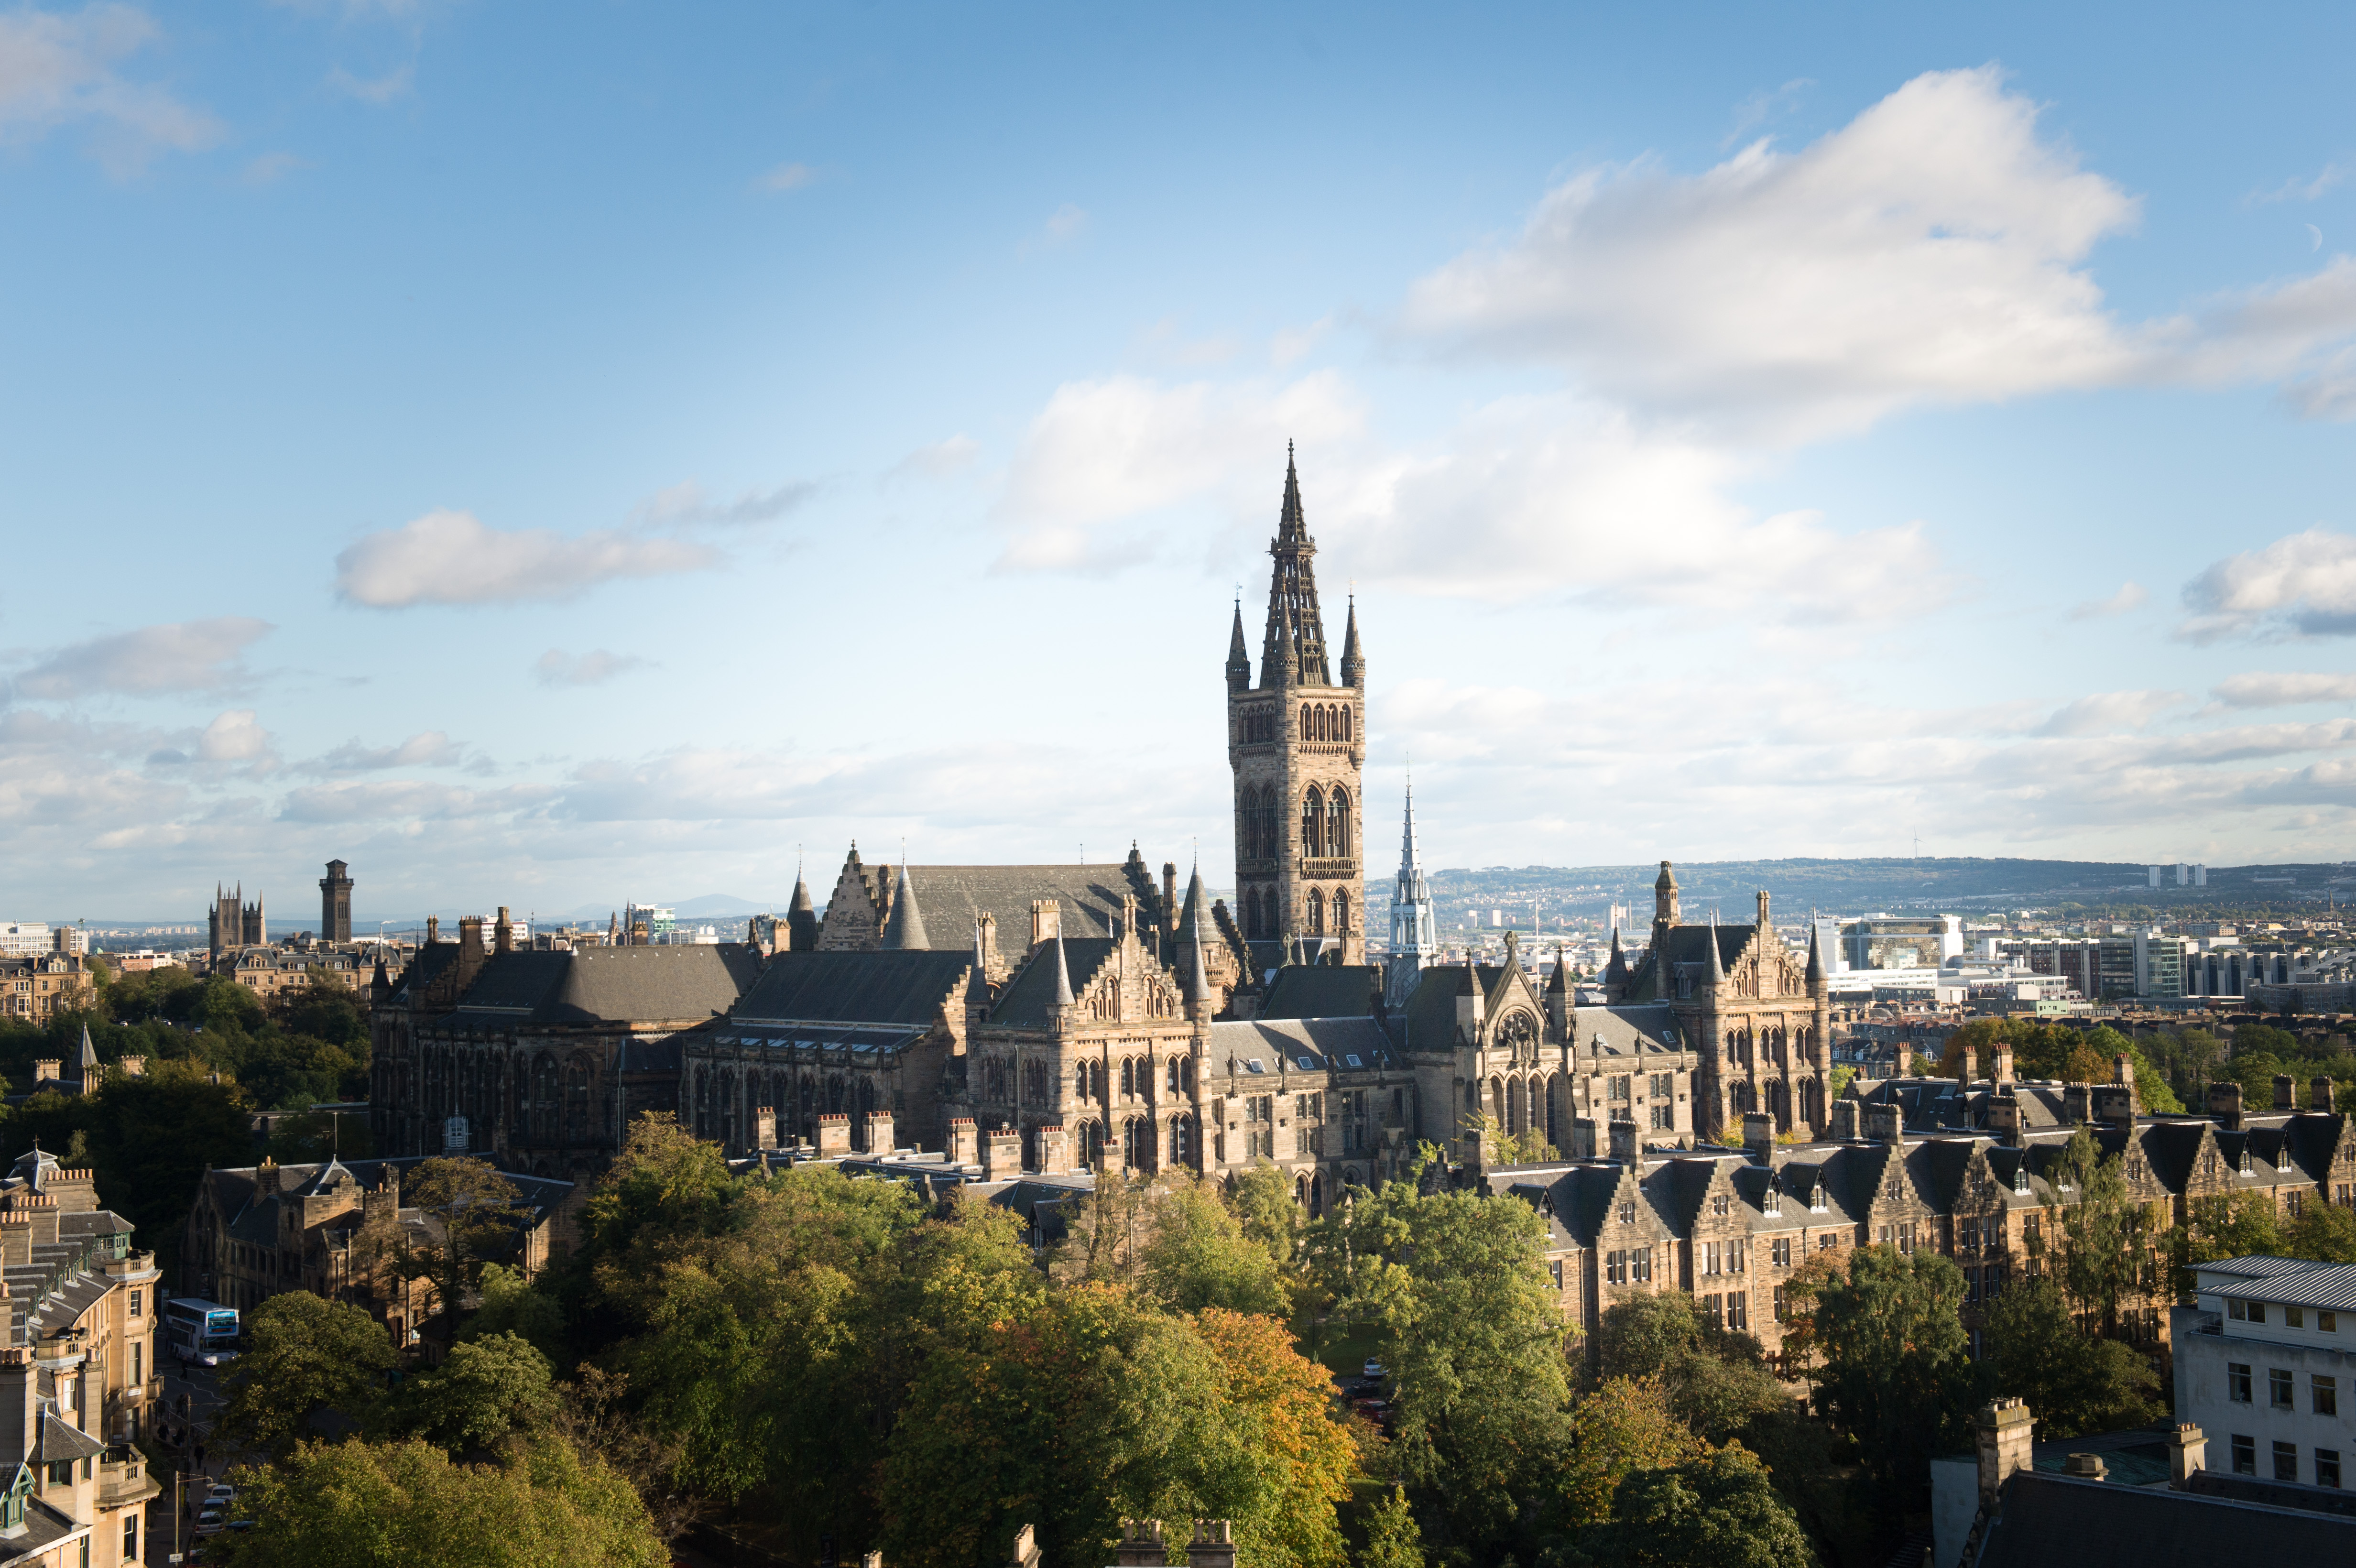
\includegraphics[keepaspectratio=true, width=\paperwidth]{../../images/background.jpg}};
    }
    \begin{frame}[plain,noframenumbering]
        \titlepage
    \end{frame}
}

\section{Finding Subgraphs}

\begin{frame}{Subgraph Isomorphism}
    \centering
    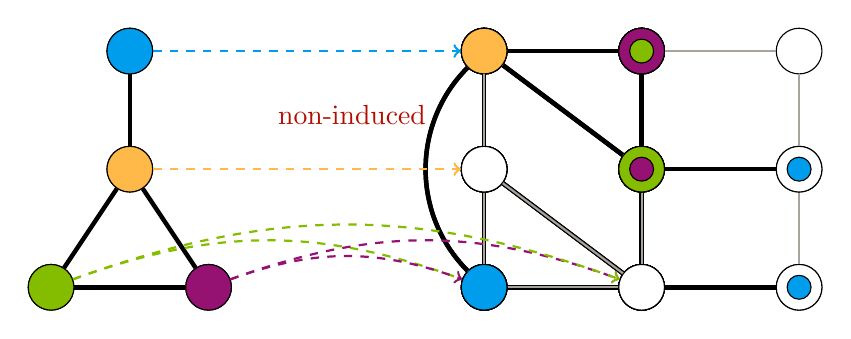
\begin{tikzpicture}
        \node <1> [draw, circle, fill=white, inner sep=4pt, font=\bfseries] (Na) at (1,  0) {\vphantom{1}};
        \node <1> [draw, circle, fill=white, inner sep=4pt, font=\bfseries] (Nb) at (1, -1.5) {\vphantom{1}};
        \node <1> [draw, circle, fill=white, inner sep=4pt, font=\bfseries] (Nc) at (0, -3) {\vphantom{1}};
        \node <1> [draw, circle, fill=white, inner sep=4pt, font=\bfseries] (Nd) at (2, -3) {\vphantom{1}};

        \node <2-> [draw, circle, fill=uofgcobalt, inner sep=4pt, font=\bfseries] (Na) at (1,  0) {\vphantom{1}};
        \node <2-> [draw, circle, fill=uofgpumpkin, inner sep=4pt, font=\bfseries] (Nb) at (1, -1.5) {\vphantom{1}};
        \node <2-> [draw, circle, fill=uofglawn, inner sep=4pt, font=\bfseries] (Nc) at (0, -3) {\vphantom{1}};
        \node <2-> [draw, circle, fill=uofgthistle, inner sep=4pt, font=\bfseries] (Nd) at (2, -3) {\vphantom{1}};

        \draw [ultra thick] (Na) -- (Nb);
        \draw [ultra thick] (Nb) -- (Nc);
        \draw [ultra thick] (Nc) -- (Nd);
        \draw [ultra thick] (Nb) -- (Nd);

        \node <1> [draw, circle, fill=white, inner sep=4pt, font=\bfseries] (N1) at (5.5,  0) {\vphantom{1}};
        \node <1> [draw, circle, fill=white, inner sep=4pt, font=\bfseries] (N2) at (7.5,  0) {\vphantom{1}};
        \node <1> [draw, circle, fill=white, inner sep=4pt, font=\bfseries] (N3) at (5.5, -1.5) {\vphantom{1}};
        \node <1> [draw, circle, fill=white, inner sep=4pt, font=\bfseries] (N4) at (7.5, -1.5) {\vphantom{1}};
        \node <1> [draw, circle, fill=white, inner sep=4pt, font=\bfseries] (N5) at (5.5, -3) {\vphantom{1}};
        \node <1> [draw, circle, fill=white, inner sep=4pt, font=\bfseries] (N6) at (7.5, -3) {\vphantom{1}};

        \node <1-6,8-> [draw, circle, fill=white, inner sep=4pt, font=\bfseries] (N7) at (9.5, -3) {\vphantom{1}};
        \node <1-4,6-> [draw, circle, fill=white, inner sep=4pt, font=\bfseries] (N8) at (9.5, -1.5) {\vphantom{1}};
        \node [draw, circle, fill=white, inner sep=4pt, font=\bfseries] (N9) at (9.5, 0) {\vphantom{1}};

        \node <2-3> [draw, circle, fill=uofgcobalt, inner sep=4pt, font=\bfseries] (N1) at (5.5,  0) {\vphantom{1}};
        \node <2-3> [draw, circle, fill=white, inner sep=4pt, font=\bfseries] (N2) at (7.5,  0) {\vphantom{1}};
        \node <2-3> [draw, circle, fill=uofgpumpkin, inner sep=4pt, font=\bfseries] (N3) at (5.5, -1.5) {\vphantom{1}};
        \node <2-3> [draw, circle, fill=white, inner sep=4pt, font=\bfseries] (N4) at (7.5, -1.5) {\vphantom{1}};
        \node <2-3> [draw, circle, fill=uofglawn, inner sep=4pt, font=\bfseries] (N5) at (5.5, -3) {\vphantom{1}};
        \node <2-3> [draw, circle, fill=uofgthistle, inner sep=4pt, font=\bfseries] (N6) at (7.5, -3) {\vphantom{1}};

        \node <4> [draw, circle, fill=uofgcobalt, inner sep=4pt, font=\bfseries] (N1) at (5.5,  0) {\vphantom{1}};
        \node <4> [draw, circle, fill=white, inner sep=4pt, font=\bfseries] (N2) at (7.5,  0) {\vphantom{1}};
        \node <4> [draw, circle, fill=uofgpumpkin, inner sep=4pt, font=\bfseries] (N3) at (5.5, -1.5) {\vphantom{1}};
        \node <4> [draw, circle, fill=white, inner sep=4pt, font=\bfseries] (N4) at (7.5, -1.5) {\vphantom{1}};
        \node <4> [draw, circle, fill=uofgthistle, inner sep=4pt, font=\bfseries] (N5) at (5.5, -3) {\vphantom{1}};
        \node <4> [draw, circle, fill=uofglawn, inner sep=4pt, font=\bfseries] (N6) at (7.5, -3) {\vphantom{1}};

        \node <5> [draw, circle, fill=uofglawn, inner sep=4pt, font=\bfseries] (N1) at (5.5,  0) {\vphantom{1}};
        \node <5> [draw, circle, fill=uofgthistle, inner sep=1pt, font=\bfseries] (N1b) at (5.5,  0) {\vphantom{1}};
        \node <5> [draw, circle, fill=uofgthistle, inner sep=4pt, font=\bfseries] (N2) at (7.5,  0) {\vphantom{1}};
        \node <5> [draw, circle, fill=uofglawn, inner sep=1pt, font=\bfseries] (N2b) at (7.5,  0) {\vphantom{1}};
        \node <5> [draw, circle, fill=white, inner sep=4pt, font=\bfseries] (N3) at (5.5, -1.5) {\vphantom{1}};
        \node <5> [draw, circle, fill=uofgpumpkin, inner sep=4pt, font=\bfseries] (N4) at (7.5, -1.5) {\vphantom{1}};
        \node <5> [draw, circle, fill=white, inner sep=4pt, font=\bfseries] (N5) at (5.5, -3) {\vphantom{1}};
        \node <5> [draw, circle, fill=white, inner sep=4pt, font=\bfseries] (N6) at (7.5, -3) {\vphantom{1}};
        \node <5> [draw, circle, fill=uofgcobalt, inner sep=1pt, font=\bfseries] (N6b) at (7.5, -3) {\vphantom{1}};
        \node <5> [draw, circle, fill=white, inner sep=4pt, font=\bfseries] (N8) at (9.5, -1.5) {\vphantom{1}};
        \node <5> [draw, circle, fill=uofgcobalt, inner sep=1pt, font=\bfseries] (N8b) at (9.5, -1.5) {\vphantom{1}};

        \node <6> [draw, circle, fill=uofgpumpkin, inner sep=4pt, font=\bfseries] (N1) at (5.5,  0) {\vphantom{1}};
        \node <6> [draw, circle, fill=uofgthistle, inner sep=4pt, font=\bfseries] (N2) at (7.5,  0) {\vphantom{1}};
        \node <6> [draw, circle, fill=uofglawn, inner sep=1pt, font=\bfseries] (N2b) at (7.5,  0) {\vphantom{1}};
        \node <6> [draw, circle, fill=uofgcobalt, inner sep=4pt, font=\bfseries] (N3) at (5.5, -1.5) {\vphantom{1}};
        \node <6> [draw, circle, fill=uofglawn, inner sep=4pt, font=\bfseries] (N4) at (7.5, -1.5) {\vphantom{1}};
        \node <6> [draw, circle, fill=uofgthistle, inner sep=1pt, font=\bfseries] (N4b) at (7.5, -1.5) {\vphantom{1}};
        \node <6> [draw, circle, fill=white, inner sep=4pt, font=\bfseries] (N5) at (5.5, -3) {\vphantom{1}};
        \node <6> [draw, circle, fill=white, inner sep=4pt, font=\bfseries] (N6) at (7.5, -3) {\vphantom{1}};

        \node <7> [draw, circle, fill=white, inner sep=4pt, font=\bfseries] (N1) at (5.5,  0) {\vphantom{1}};
        \node <7> [draw, circle, fill=white, inner sep=4pt, font=\bfseries] (N2) at (7.5,  0) {\vphantom{1}};
        \node <7> [draw, circle, fill=uofgthistle, inner sep=4pt, font=\bfseries] (N3) at (5.5, -1.5) {\vphantom{1}};
        \node <7> [draw, circle, fill=uofglawn, inner sep=1pt, font=\bfseries] (N3b) at (5.5, -1.5) {\vphantom{1}};
        \node <7> [draw, circle, fill=white, inner sep=4pt, font=\bfseries] (N4) at (7.5, -1.5) {\vphantom{1}};
        \node <7> [draw, circle, fill=uofgcobalt, inner sep=1pt, font=\bfseries] (N4b) at (7.5, -1.5) {\vphantom{1}};
        \node <7> [draw, circle, fill=uofglawn, inner sep=4pt, font=\bfseries] (N5) at (5.5, -3) {\vphantom{1}};
        \node <7> [draw, circle, fill=uofgthistle, inner sep=1pt, font=\bfseries] (N5b) at (5.5, -3) {\vphantom{1}};
        \node <7> [draw, circle, fill=uofgpumpkin, inner sep=4pt, font=\bfseries] (N6) at (7.5, -3) {\vphantom{1}};
        \node <7> [draw, circle, fill=white, inner sep=4pt, font=\bfseries] (N7) at (9.5, -3) {\vphantom{1}};
        \node <7> [draw, circle, fill=uofgcobalt, inner sep=1pt, font=\bfseries] (N7b) at (9.5, -3) {\vphantom{1}};

        \node <8> [draw, circle, fill=uofgcobalt, inner sep=4pt, font=\bfseries] (N1) at (5.5,  0) {\vphantom{1}};
        \node <8> [draw, circle, fill=white, inner sep=4pt, font=\bfseries] (N2) at (7.5,  0) {\vphantom{1}};
        \node <8> [draw, circle, fill=uofglawn, inner sep=4pt, font=\bfseries] (N3) at (5.5, -1.5) {\vphantom{1}};
        \node <8> [draw, circle, fill=uofgthistle, inner sep=1pt, font=\bfseries] (N3b) at (5.5, -1.5) {\vphantom{1}};
        \node <8> [draw, circle, fill=white, inner sep=4pt, font=\bfseries] (N4) at (7.5, -1.5) {\vphantom{1}};
        \node <8> [draw, circle, fill=uofgpumpkin, inner sep=4pt, font=\bfseries] (N5) at (5.5, -3) {\vphantom{1}};
        \node <8> [draw, circle, fill=uofgthistle, inner sep=4pt, font=\bfseries] (N6) at (7.5, -3) {\vphantom{1}};
        \node <8> [draw, circle, fill=uofglawn, inner sep=1pt, font=\bfseries] (N6b) at (7.5, -3) {\vphantom{1}};

        \node <9-> [draw, circle, fill=uofgpumpkin, inner sep=4pt, font=\bfseries] (N1) at (5.5,  0) {\vphantom{1}};
        \node <9-> [draw, circle, fill=uofgthistle, inner sep=4pt, font=\bfseries] (N2) at (7.5,  0) {\vphantom{1}};
        \node <9-> [draw, circle, fill=uofglawn, inner sep=1pt, font=\bfseries] (N2b) at (7.5,  0) {\vphantom{1}};
        \node <9-> [draw, circle, fill=white, inner sep=4pt, font=\bfseries] (N3) at (5.5, -1.5) {\vphantom{1}};
        \node <9-> [draw, circle, fill=uofglawn, inner sep=4pt, font=\bfseries] (N4) at (7.5, -1.5) {\vphantom{1}};
        \node <9-> [draw, circle, fill=uofgthistle, inner sep=1pt, font=\bfseries] (N4b) at (7.5, -1.5) {\vphantom{1}};
        \node <9-> [draw, circle, fill=uofgcobalt, inner sep=4pt, font=\bfseries] (N5) at (5.5, -3) {\vphantom{1}};
        \node <9-> [draw, circle, fill=white, inner sep=4pt, font=\bfseries] (N6) at (7.5, -3) {\vphantom{1}};

        \draw <1> [thick, color=uofgsandstone!50] (N1) -- (N2);
        \draw <1> [thick, color=uofgsandstone!50] (N1) -- (N3);
        \draw <1> [thick, color=uofgsandstone!50] (N1) -- (N4);
        \draw <1> [thick, color=uofgsandstone!50] (N2) -- (N4);
        \draw <1> [thick, color=uofgsandstone!50] (N3) -- (N5);
        \draw <1> [thick, color=uofgsandstone!50] (N3) -- (N6);
        \draw <1> [thick, color=uofgsandstone!50] (N4) -- (N6);
        \draw <1> [thick, color=uofgsandstone!50] (N5) -- (N6);
        \draw <1> [thick, color=uofgsandstone!50] (N1) to [in=135, out=225] (N5);

        \draw <2-4> [thick, color=uofgsandstone!50] (N1) -- (N2);
        \draw <2-4> [ultra thick] (N1) -- (N3);
        \draw <2-4> [thick, color=uofgsandstone!50] (N1) -- (N4);
        \draw <2-4> [thick, color=uofgsandstone!50] (N2) -- (N4);
        \draw <2-4> [ultra thick] (N3) -- (N5);
        \draw <2-4> [ultra thick] (N3) -- (N6);
        \draw <2-4> [thick, color=uofgsandstone!50] (N4) -- (N6);
        \draw <2-4> [ultra thick] (N5) -- (N6);
        \draw <2> [thick, color=uofgsandstone!50] (N1) to [in=135, out=225] (N5);
        \draw <3> [thick, color=uofgpillarbox] (N1) to [in=135, out=225] node [near start, left] { non-induced } (N5);
        \draw <4> [thick, color=uofgsandstone!50] (N1) to [in=135, out=225] (N5);

        \draw <5> [ultra thick] (N1) -- (N2);
        \draw <5> [thick, color=uofgsandstone!50] (N1) -- (N3);
        \draw <5> [ultra thick] (N1) -- (N4);
        \draw <5> [ultra thick] (N2) -- (N4);
        \draw <5> [thick, color=uofgsandstone!50] (N3) -- (N5);
        \draw <5> [thick, color=uofgsandstone!50] (N3) -- (N6);
        \draw <5> [ultra thick] (N4) -- (N6);
        \draw <5> [thick, color=uofgsandstone!50] (N5) -- (N6);
        \draw <5> [thick, color=uofgsandstone!50] (N1) to [in=135, out=225] (N5);

        \draw <6> [ultra thick] (N1) -- (N2);
        \draw <6> [ultra thick] (N1) -- (N3);
        \draw <6> [ultra thick] (N1) -- (N4);
        \draw <6> [ultra thick] (N2) -- (N4);
        \draw <6> [thick, color=uofgsandstone!50] (N3) -- (N5);
        \draw <6> [thick, color=uofgsandstone!50] (N3) -- (N6);
        \draw <6> [thick, color=uofgsandstone!50] (N4) -- (N6);
        \draw <6> [thick, color=uofgsandstone!50] (N5) -- (N6);
        \draw <6> [thick, color=uofgsandstone!50] (N1) to [in=135, out=225] (N5);

        \draw <7> [thick, color=uofgsandstone!50] (N1) -- (N2);
        \draw <7> [thick, color=uofgsandstone!50] (N1) -- (N3);
        \draw <7> [thick, color=uofgsandstone!50] (N1) -- (N4);
        \draw <7> [thick, color=uofgsandstone!50] (N2) -- (N4);
        \draw <7> [ultra thick] (N3) -- (N5);
        \draw <7> [ultra thick] (N3) -- (N6);
        \draw <7> [ultra thick] (N4) -- (N6);
        \draw <7> [ultra thick] (N5) -- (N6);
        \draw <7> [thick, color=uofgsandstone!50] (N1) to [in=135, out=225] (N5);

        \draw <8> [thick, color=uofgsandstone!50] (N1) -- (N2);
        \draw <8> [thick, color=uofgsandstone!50] (N1) -- (N3);
        \draw <8> [thick, color=uofgsandstone!50] (N1) -- (N4);
        \draw <8> [thick, color=uofgsandstone!50] (N2) -- (N4);
        \draw <8> [ultra thick] (N3) -- (N5);
        \draw <8> [ultra thick] (N3) -- (N6);
        \draw <8> [thick, color=uofgsandstone!50] (N4) -- (N6);
        \draw <8> [ultra thick] (N5) -- (N6);
        \draw <8> [ultra thick] (N1) to [in=135, out=225] (N5);

        \draw <9-> [ultra thick] (N1) -- (N2);
        \draw <9-> [thick, color=uofgsandstone!50] (N1) -- (N3);
        \draw <9-> [ultra thick] (N1) -- (N4);
        \draw <9-> [ultra thick] (N2) -- (N4);
        \draw <9-> [thick, color=uofgsandstone!50] (N3) -- (N5);
        \draw <9-> [thick, color=uofgsandstone!50] (N3) -- (N6);
        \draw <9-> [thick, color=uofgsandstone!50] (N4) -- (N6);
        \draw <9-> [thick, color=uofgsandstone!50] (N5) -- (N6);
        \draw <9-> [ultra thick] (N1) to [in=135, out=225] (N5);

        \draw <2-3> [thick, dashed, color=uofgcobalt, arrows=->] (Na) to (N1);
        \draw <2-3> [thick, dashed, color=uofgpumpkin, arrows=->] (Nb) to (N3);
        \draw <2-3> [thick, dashed, color=uofglawn, arrows=->] (Nc) to [out=20, in=160] (N5);
        \draw <2-3> [thick, dashed, color=uofgthistle, arrows=->] (Nd) to [out=20, in=160] (N6);

        \draw <4> [thick, dashed, color=uofgcobalt, arrows=->] (Na) to (N1);
        \draw <4> [thick, dashed, color=uofgpumpkin, arrows=->] (Nb) to (N3);
        \draw <4> [thick, dashed, color=uofglawn, arrows=->] (Nc) to [out=20, in=160] (N6);
        \draw <4> [thick, dashed, color=uofgthistle, arrows=->] (Nd) to [out=20, in=160] (N5);

        \draw [thick, color=uofgsandstone!50] (N7) -- (N8);
        \draw [thick, color=uofgsandstone!50] (N8) -- (N9);
        \draw [thick, color=uofgsandstone!50] (N2) -- (N9);
        \draw <1-4,6-> [thick, color=uofgsandstone!50] (N4) -- (N8);
        \draw <5> [ultra thick] (N4) -- (N8);
        \draw <1-6,8-> [thick, color=uofgsandstone!50] (N6) -- (N7);
        \draw <7> [ultra thick] (N6) -- (N7);
    \end{tikzpicture}

    \uncover<10->{

        \bigskip

        How many did I miss?
    }
\end{frame}

\begin{frame}{Maximum Common Induced Subgraph}
    \centering
    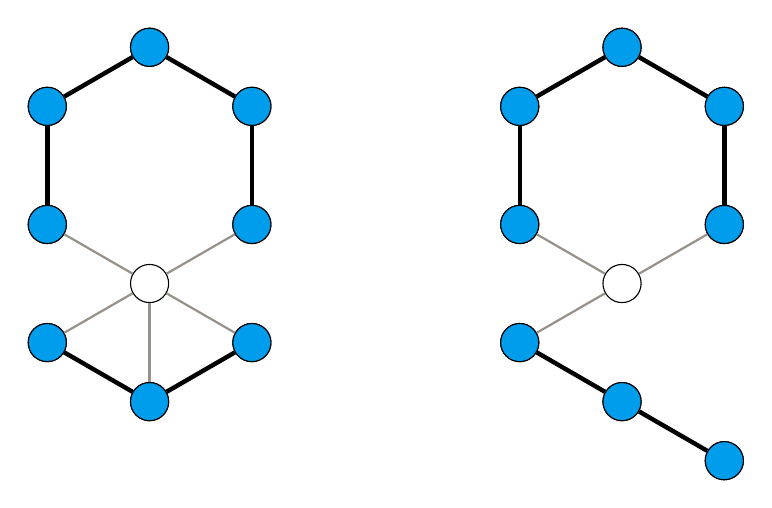
\begin{tikzpicture}
        \begin{scope}
            \node<1> [draw, circle, inner sep=2pt, font=\normalsize] (M1) at (90:1.5) {\phantom{0}};
            \node<2> [draw, circle, fill=uofgcobalt, inner sep=2pt, font=\normalsize] (M1) at (90:1.5) {\phantom{0}};
            \node<1> [draw, circle, inner sep=2pt, font=\normalsize] (M2) at (150:1.5) {\phantom{0}};
            \node<2> [draw, circle, fill=uofgcobalt, inner sep=2pt, font=\normalsize] (M2) at (150:1.5) {\phantom{0}};
            \node<1> [draw, circle, inner sep=2pt, font=\normalsize] (M3) at (30:1.5) {\phantom{0}};
            \node<2> [draw, circle, fill=uofgcobalt, inner sep=2pt, font=\normalsize] (M3) at (30:1.5) {\phantom{0}};
            \node<1> [draw, circle, inner sep=2pt, font=\normalsize] (M4) at (210:1.5) {\phantom{0}};
            \node<2> [draw, circle, fill=uofgcobalt, inner sep=2pt, font=\normalsize] (M4) at (210:1.5) {\phantom{0}};
            \node<1> [draw, circle, inner sep=2pt, font=\normalsize] (M5) at (330:1.5) {\phantom{0}};
            \node<2> [draw, circle, fill=uofgcobalt, inner sep=2pt, font=\normalsize] (M5) at (330:1.5) {\phantom{0}};
            \node[draw, circle, fill=white, inner sep=2pt, font=\normalsize] (M6) at (270:1.5) {\phantom{0}};
            \node<1> [draw, circle, inner sep=2pt, font=\normalsize] (M7) at ($(210:1.5) + (M6)$) {\phantom{0}};
            \node<2> [draw, circle, fill=uofgcobalt, inner sep=2pt, font=\normalsize] (M7) at ($(210:1.5) + (M6)$) {\phantom{0}};
            \node<1> [draw, circle, inner sep=2pt, font=\normalsize] (M8) at ($(330:1.5) + (M6)$) {\phantom{0}};
            \node<2> [draw, circle, fill=uofgcobalt, inner sep=2pt, font=\normalsize] (M8) at ($(330:1.5) + (M6)$) {\phantom{0}};
            \node<1> [draw, circle, inner sep=2pt, font=\normalsize] (M9) at ($(270:1.5) + (M6)$) {\phantom{0}};
            \node<2> [draw, circle, fill=uofgcobalt, inner sep=2pt, font=\normalsize] (M9) at ($(270:1.5) + (M6)$) {\phantom{0}};

            \draw<1> [thick, color=uofgsandstone!60] (M1) -- (M2);
            \draw<2> [ultra thick] (M1) -- (M2);
            \draw<1> [thick, color=uofgsandstone!60] (M2) -- (M4);
            \draw<2> [ultra thick] (M2) -- (M4);
            \draw<1> [thick, color=uofgsandstone!60] (M3) -- (M5);
            \draw<2> [ultra thick] (M3) -- (M5);
            \draw [thick, color=uofgsandstone!60] (M4) -- (M6);
            \draw [thick, color=uofgsandstone!60] (M5) -- (M6);
            \draw<1> [thick, color=uofgsandstone!60] (M3) -- (M1);
            \draw<2> [ultra thick] (M3) -- (M1);
            \draw [thick, color=uofgsandstone!60] (M6) -- (M7);
            \draw [thick, color=uofgsandstone!60] (M6) -- (M8);
            \draw [thick, color=uofgsandstone!60] (M6) -- (M9);
            \draw<1> [thick, color=uofgsandstone!60] (M7) -- (M9);
            \draw<2> [ultra thick] (M7) -- (M9);
            \draw<1> [thick, color=uofgsandstone!60] (M8) -- (M9);
            \draw<2> [ultra thick] (M8) -- (M9);
        \end{scope}

        \begin{scope}[xshift=6cm]
            \node<1> [draw, circle, inner sep=2pt, font=\normalsize] (M1) at (90:1.5) {\phantom{0}};
            \node<2> [draw, circle, fill=uofgcobalt, inner sep=2pt, font=\normalsize] (M1) at (90:1.5) {\phantom{0}};
            \node<1> [draw, circle, inner sep=2pt, font=\normalsize] (M2) at (150:1.5) {\phantom{0}};
            \node<2> [draw, circle, fill=uofgcobalt, inner sep=2pt, font=\normalsize] (M2) at (150:1.5) {\phantom{0}};
            \node<1> [draw, circle, inner sep=2pt, font=\normalsize] (M3) at (30:1.5) {\phantom{0}};
            \node<2> [draw, circle, fill=uofgcobalt, inner sep=2pt, font=\normalsize] (M3) at (30:1.5) {\phantom{0}};
            \node<1> [draw, circle, inner sep=2pt, font=\normalsize] (M4) at (210:1.5) {\phantom{0}};
            \node<2> [draw, circle, fill=uofgcobalt, inner sep=2pt, font=\normalsize] (M4) at (210:1.5) {\phantom{0}};
            \node<1> [draw, circle, inner sep=2pt, font=\normalsize] (M5) at (330:1.5) {\phantom{0}};
            \node<2> [draw, circle, fill=uofgcobalt, inner sep=2pt, font=\normalsize] (M5) at (330:1.5) {\phantom{0}};
            \node[draw, circle, fill=white, inner sep=2pt, font=\normalsize] (M6) at (270:1.5) {\phantom{0}};
            \node<1> [draw, circle, inner sep=2pt, font=\normalsize] (M7) at ($(210:1.5) + (M6)$) {\phantom{0}};
            \node<2> [draw, circle, fill=uofgcobalt, inner sep=2pt, font=\normalsize] (M7) at ($(210:1.5) + (M6)$) {\phantom{0}};
            \node<1> [draw, circle, inner sep=2pt, font=\normalsize] (M8) at ($(270:1.5) + (M6)$) {\phantom{0}};
            \node<2> [draw, circle, fill=uofgcobalt, inner sep=2pt, font=\normalsize] (M8) at ($(270:1.5) + (M6)$) {\phantom{0}};
            \node<1> [draw, circle, inner sep=2pt, font=\normalsize] (M9) at ($(330:1.5) + (M8)$) {\phantom{0}};
            \node<2> [draw, circle, fill=uofgcobalt, inner sep=2pt, font=\normalsize] (M9) at ($(330:1.5) + (M8)$) {\phantom{0}};

            \draw<1> [thick, color=uofgsandstone!60] (M1) -- (M2);
            \draw<2> [ultra thick] (M1) -- (M2);
            \draw<1> [thick, color=uofgsandstone!60] (M2) -- (M4);
            \draw<2> [ultra thick] (M2) -- (M4);
            \draw<1> [thick, color=uofgsandstone!60] (M3) -- (M5);
            \draw<2> [ultra thick] (M3) -- (M5);
            \draw [thick, color=uofgsandstone!60] (M4) -- (M6);
            \draw [thick, color=uofgsandstone!60] (M5) -- (M6);
            \draw<1> [thick, color=uofgsandstone!60] (M3) -- (M1);
            \draw<2> [ultra thick] (M3) -- (M1);
            \draw [thick, color=uofgsandstone!60] (M6) -- (M7);
            \draw<1> [thick, color=uofgsandstone!60] (M7) -- (M8);
            \draw<2> [ultra thick] (M7) -- (M8);
            \draw<1> [thick, color=uofgsandstone!60] (M8) -- (M9);
            \draw<2> [ultra thick] (M8) -- (M9);
        \end{scope}
    \end{tikzpicture}
\end{frame}

\begin{frame}{Maximum Common Induced Connected Subgraph}
    \centering
    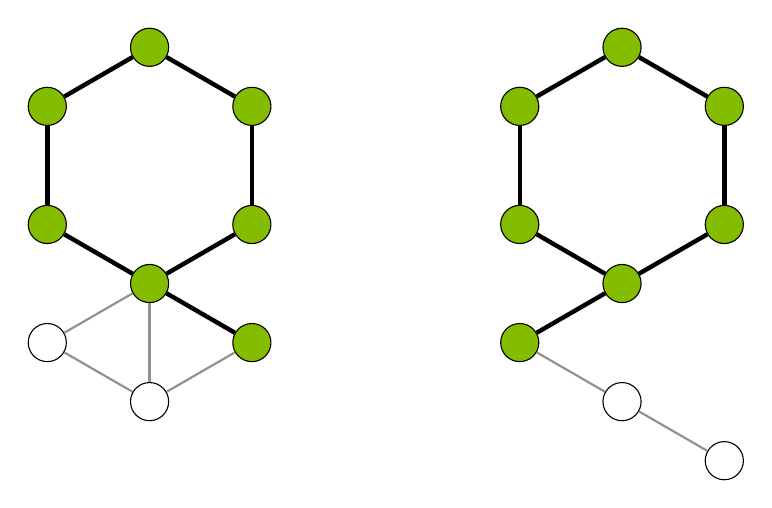
\begin{tikzpicture}
        \begin{scope}
            \node[draw, circle, fill=uofglawn, inner sep=2pt, font=\normalsize] (M1) at (90:1.5) {\phantom{0}};
            \node[draw, circle, fill=uofglawn, inner sep=2pt, font=\normalsize] (M2) at (150:1.5) {\phantom{0}};
            \node[draw, circle, fill=uofglawn, inner sep=2pt, font=\normalsize] (M3) at (30:1.5) {\phantom{0}};
            \node[draw, circle, fill=uofglawn, inner sep=2pt, font=\normalsize] (M4) at (210:1.5) {\phantom{0}};
            \node[draw, circle, fill=uofglawn, inner sep=2pt, font=\normalsize] (M5) at (330:1.5) {\phantom{0}};
            \node[draw, circle, fill=uofglawn, inner sep=2pt, font=\normalsize] (M6) at (270:1.5) {\phantom{0}};
            \node[draw, circle, fill=white, inner sep=2pt, font=\normalsize] (M7) at ($(210:1.5) + (M6)$) {\phantom{0}};
            \node[draw, circle, fill=uofglawn, inner sep=2pt, font=\normalsize] (M8) at ($(330:1.5) + (M6)$) {\phantom{0}};
            \node[draw, circle, fill=white, inner sep=2pt, font=\normalsize] (M9) at ($(270:1.5) + (M6)$) {\phantom{0}};

            \draw [ultra thick] (M1) -- (M2);
            \draw [ultra thick] (M2) -- (M4);
            \draw [ultra thick] (M3) -- (M5);
            \draw [ultra thick] (M4) -- (M6);
            \draw [ultra thick] (M5) -- (M6);
            \draw [ultra thick] (M3) -- (M1);
            \draw [thick, color=uofgsandstone!60] (M6) -- (M7);
            \draw [ultra thick] (M6) -- (M8);
            \draw [thick, color=uofgsandstone!60] (M6) -- (M9);
            \draw [thick, color=uofgsandstone!60] (M7) -- (M9);
            \draw [thick, color=uofgsandstone!60] (M8) -- (M9);
        \end{scope}

        \begin{scope}[xshift=6cm]
            \node[draw, circle, fill=uofglawn, inner sep=2pt, font=\normalsize] (M1) at (90:1.5) {\phantom{0}};
            \node[draw, circle, fill=uofglawn, inner sep=2pt, font=\normalsize] (M2) at (150:1.5) {\phantom{0}};
            \node[draw, circle, fill=uofglawn, inner sep=2pt, font=\normalsize] (M3) at (30:1.5) {\phantom{0}};
            \node[draw, circle, fill=uofglawn, inner sep=2pt, font=\normalsize] (M4) at (210:1.5) {\phantom{0}};
            \node[draw, circle, fill=uofglawn, inner sep=2pt, font=\normalsize] (M5) at (330:1.5) {\phantom{0}};
            \node[draw, circle, fill=uofglawn, inner sep=2pt, font=\normalsize] (M6) at (270:1.5) {\phantom{0}};
            \node[draw, circle, fill=uofglawn, inner sep=2pt, font=\normalsize] (M7) at ($(210:1.5) + (M6)$) {\phantom{0}};
            \node[draw, circle, fill=white, inner sep=2pt, font=\normalsize] (M8) at ($(270:1.5) + (M6)$) {\phantom{0}};
            \node[draw, circle, fill=white, inner sep=2pt, font=\normalsize] (M9) at ($(330:1.5) + (M8)$) {\phantom{0}};

            \draw [ultra thick] (M1) -- (M2);
            \draw [ultra thick] (M2) -- (M4);
            \draw [ultra thick] (M3) -- (M5);
            \draw [ultra thick] (M4) -- (M6);
            \draw [ultra thick] (M5) -- (M6);
            \draw [ultra thick] (M3) -- (M1);
            \draw [ultra thick] (M6) -- (M7);
            \draw [thick, draw=uofgsandstone!60] (M7) -- (M8);
            \draw [thick, draw=uofgsandstone!60] (M8) -- (M9);
        \end{scope}
    \end{tikzpicture}
\end{frame}

\begin{frame}{Maximum Clique}
    \centering
    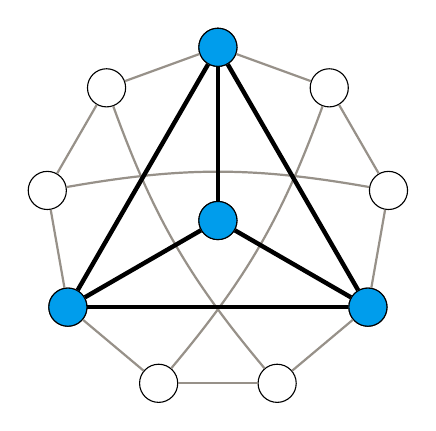
\begin{tikzpicture}
        \newcount \myc
        \foreach \n in {1, ..., 9}{
            \myc=\n \advance\myc by -1 \multiply\myc by -360 \divide\myc by 9 \advance\myc by 290
            \ifthenelse{\n = 3 \OR \n = 6 \OR \n = 9}{
                \node<1>[draw, circle, inner sep=2pt] (N\n) at (\the\myc:2.2) {\phantom{0}};
                \node<2>[draw, circle, fill=uofgcobalt, inner sep=2pt] (N\n) at (\the\myc:2.2) {\phantom{0}};
            }{
                \node[draw, circle, fill=white, inner sep=2pt] (N\n) at (\the\myc:2.2) {\phantom{0}};
            }
        }
        \node<1>[draw, circle, inner sep=2pt] (N10) at (0, 0) {\phantom{0}};
        \node<2>[draw, circle, fill=uofgcobalt, inner sep=2pt] (N10) at (0, 0) {\phantom{0}};

        \draw [thick, color=uofgsandstone!60] (N1) -- (N2);
        \draw [thick, color=uofgsandstone!60] (N2) -- (N3);
        \draw [thick, color=uofgsandstone!60] (N3) -- (N4);
        \draw [thick, color=uofgsandstone!60] (N4) -- (N5);
        \draw [thick, color=uofgsandstone!60] (N5) -- (N6);
        \draw [thick, color=uofgsandstone!60] (N6) -- (N7);
        \draw [thick, color=uofgsandstone!60] (N7) -- (N8);
        \draw [thick, color=uofgsandstone!60] (N8) -- (N9);
        \draw [thick, color=uofgsandstone!60] (N9) -- (N1);

        \draw [thick, color=uofgsandstone!60] (N4) to [out=10, in=170] (N8);
        \draw [thick, color=uofgsandstone!60] (N2) to [out=50, in=250] (N7);
        \draw [thick, color=uofgsandstone!60] (N5) to [out=290, in=130] (N1);

        \draw<1> [thick, color=uofgsandstone!60] (N3) -- (N10);
        \draw<2> [ultra thick] (N3) -- (N10);
        \draw<1> [thick, color=uofgsandstone!60] (N6) -- (N10);
        \draw<2> [ultra thick] (N6) -- (N10);
        \draw<1> [thick, color=uofgsandstone!60] (N9) -- (N10);
        \draw<2> [ultra thick] (N9) -- (N10);
        \draw<1> [thick, color=uofgsandstone!60] (N6) -- (N3);
        \draw<2> [ultra thick] (N6) -- (N3);
        \draw<1> [thick, color=uofgsandstone!60] (N9) -- (N3);
        \draw<2> [ultra thick] (N9) -- (N3);
        \draw<1> [thick, color=uofgsandstone!60] (N6) -- (N9);
        \draw<2> [ultra thick] (N6) -- (N9);
    \end{tikzpicture}
\end{frame}

\begin{frame}{Who Cares?}
    \begin{itemize}
        \item Chemistry, biochemistry, and drug design (graphs are molecule fragments or proteins).
        \item Computer vision.
        \item Compilers (instruction generation, code rewriting).
        \item Plagiarism and malware detection.
        \item Livestock epidemiology (contact and trade graphs).
        \item Designing mechanical lock systems.
    \end{itemize}
\end{frame}

\begin{frame}{In Theory\ldots}
    \begin{itemize}
        \item Subgraph finding is hard.
        \item Subgraph counting is hard.
        \item Approximate subgraph finding is hard.
    \end{itemize}
\end{frame}

\begin{frame}{In Practice\ldots}
    \begin{itemize}
        \item We have good \emph{solvers} for subgraph problems.
        \item Some applications involve solving thousands of subgraph isomorphism queries per second.
        \item We can solve clique on larger graphs than we can solve all-pairs
            shortest path.\footnote{Terms and conditions apply.}
        \item<2-> Maximum common subgraph is still a nightmare\ldots
        \item<3-> People often don't actually want to solve simple subgraph isomorphism.
    \end{itemize}
\end{frame}

\begin{frame}{Graphs Aren't Just Graphs}
    \begin{itemize}
        \item Vertex and / or edge labels, or broader compatibility functions.
        \item Directed edges.
        \item Multi-edges, more than one edge between vertices.
        \item Hyper-edges, between more than two vertices.
        \item Partially defined graphs?
        \item No need for injectivity (homomorphism), or only local injectivity.
        \item <2-> Don't forget about loops!
        \item <3-> Might want all solutions, or a count.
    \end{itemize}
\end{frame}

\section{Algorithm Basics}

\begin{frame}{Two Solver Design Philosophies}
    \begin{enumerate}
        \item Pick a vertex, guess where it goes, and start trying to grow a connected component.
            \begin{itemize}
                \item Popular solvers: VF2, VF3, RI, TurboISO, \ldots
                \item Very fast to start up.
                \item Often good on easy instances.
                \item Spectacularly bad on hard instances, and on some easy instances.
            \end{itemize}
        \item Use constraint programming, build a mapping from the pattern graph to the target
            graph.
            \begin{itemize}
                \item LAD, Glasgow Subgraph Solver.
                \item Consistent performance on easy instances.
                \item Much better on hard instances.
            \end{itemize}
    \end{enumerate}
\end{frame}

\subsection{McCreesh, Prosser, Trimble: The Glasgow Subgraph Solver: Using
Constraint Programming to Tackle Hard Subgraph Isomorphism Problem Variants. ICGT 2020}

\begin{frame}{The Glasgow Subgraph Solver}
    \begin{center}
        \url{https://github.com/ciaranm/glasgow-subgraph-solver}
    \end{center}

    \begin{itemize}
        \item A CP style solver specifically for subgraph algorithms.
        \item Subgraph isomorphism, and all its variants (induced / non-induced, homomorphism,
            locally injective, labels, side constraints, directed, \ldots).
        \item Also special algorithms for clique.
        \item Guaranteed no bugs!
            \begin{itemize}
                \item<2-> Or at least, any buggy output will always be detected, if you enable proof
                    logging.
            \end{itemize}
    \end{itemize}
\end{frame}

\subsection{Solnon: Empirical Evaluation of Subgraph Isomorphism Solvers. GbRPR 2019}

\begin{frame}{Benchmark Instances}
    \begin{center}
        \url{http://perso.citi-lab.fr/csolnon/SIP.html}
    \end{center}

    \begin{itemize}
        \item 14,621 instances from Christine Solnon's collection:
            \begin{itemize}
                \item Randomly generated with different models (MIVIA suite).
                \item Real-world graphs.
                \item Computer vision problems.
                \item Biochemistry problems.
                \item Phase transition instances.
            \end{itemize}
        \item At least\ldots
            \begin{itemize}
                \item $\ge$ 2,110 satisfiable.
                \item $\ge$ 12,322 unsatisfiable.
            \end{itemize}
        \item A lot of them are very easy for good algorithms.
    \end{itemize}
\end{frame}

\begin{frame}{Is It Any Good?}

    \centering
    \includegraphics<1>{gen-graph-others.pdf}%

\end{frame}

\begin{frame}{Easy Conclusion!}
    \begin{itemize}
        \item CP is best!
    \end{itemize}
\end{frame}

\subsection{McCreesh, Prosser, Solnon, Trimble: When Subgraph Isomorphism is Really Hard, and Why
This Matters for Graph Databases. JAIR 61 (2018)}

\begin{frame}{An Observation about Certain Datasets}
    \begin{itemize}
        \item All of the randomly generated instances from the MIVIA suites are satisfiable.
        \item The target graphs are randomly generated, and patterns are made by selecting
            random connected subgraphs and permuting them.
        \item These instances are usually rather easy\ldots
        \item Many papers use \emph{only} these instances for benchmarking.
    \end{itemize}
\end{frame}

\begin{frame}{A Different Easy Conclusion!}
    \begin{itemize}
        \item CP is slow! RI is best!
    \end{itemize}
\end{frame}

\subsection{McCreesh, Prosser, Trimble: The Glasgow Subgraph Solver: Using
Constraint Programming to Tackle Hard Subgraph Isomorphism Problem Variants. ICGT 2020}

\begin{frame}{Constraint Programming}
    \begin{itemize}
        \item We have some \textcolor{uofgcobalt}{variables}, each of which has a
            \textcolor{uofgcobalt}{domain} of possible \textcolor{uofgcobalt}{values}.
        \item Give each variable a value from its domain, whilst respecting all
            \textcolor{uofgcobalt}{constraints}.
    \end{itemize}
\end{frame}

\begin{frame}{Building a Mapping}
    \begin{itemize}
        \item One variable per pattern vertex.
        \item Domains and values are target vertices.
        \item We think of these variables as defining a function.
    \end{itemize}
\end{frame}

\begin{frame}{Injectivity}
    \begin{itemize}
        \item Can't map to the same target vertex twice.
        \item Could say that each pair of pattern vertices are not equal?
        \item <2-> We prefer high-level constraints, so we just say ``all different''.
    \end{itemize}
\end{frame}

\begin{frame}{Adjacency}
    \begin{itemize}
        \item If A and B are adjacent in the pattern, $f(A)$ must be adjacent to $f(B)$
            in the target.
        \item Various ways of encoding this. In SAT we'd need $n^4$ clauses, or $n^3$ if
            we're sneaky.
        \item In practice: we write a special constraint propagator to do this efficiently.
    \end{itemize}
\end{frame}

\begin{frame}{Backtracking Search, Maintaining Consistency}
    \begin{itemize}
        \item Pick a variable $V$ that has more than one value remaining.
        \item For each of its values $v$ in turn:
            \begin{itemize}
                \item Try $V = v$, and do some inference.
                    \begin{itemize}
                        \item No other variable can take the value $v$.
                        \item Variables adjacent to $V$ must be given values adjacent to $v$.
                    \end{itemize}
                \item If we get an empty domain, we made a bad guess.
                \item If every variable has one value left, we have a solution.
                \item Otherwise, recurse.
            \end{itemize}
    \end{itemize}
\end{frame}

\begin{frame}{Data Structures}
    \begin{itemize}
        \item We store a set of values for every variable.
        \item Need to be able to test whether a specific value is present, remove values,
            count how many values remain.
        \item Must either be copyable, or have some way of doing backtracking.
        \item <2-> Objectively correct answer: bitsets.
    \end{itemize}
\end{frame}

\section{Filtering}

\subsection{McCreesh, Prosser, Trimble: The Glasgow Subgraph Solver: Using
Constraint Programming to Tackle Hard Subgraph Isomorphism Problem Variants. ICGT 2020}

\begin{frame}{Degree Filtering}
    \begin{itemize}
        \item Can't map a vertex of degree $d$ to a vertex of degree less than $d$.
    \end{itemize}

    \bigskip

    \centering
    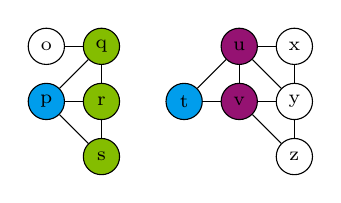
\begin{tikzpicture}
        \node [draw, circle, fill=white, inner sep=2.5pt, font=\scriptsize] (NO) at (0, 0.7) {\phantom{1}};
        \node [anchor=center, font=\scriptsize] at (NO) {o};
        \node [draw, circle, fill=uofgcobalt, inner sep=2.5pt, font=\scriptsize] (NP) at (0, 0) {\phantom{1}};
        \node [anchor=center, font=\scriptsize] at (NP) {p};
        \node [draw, circle, fill=uofglawn, inner sep=2.5pt, font=\scriptsize] (NQ) at (0.7, 0.7) {\phantom{1}};
        \node [anchor=center, font=\scriptsize] at (NQ) {q};
        \node [draw, circle, fill=uofglawn, inner sep=2.5pt, font=\scriptsize] (NR) at (0.7, 0) {\phantom{1}};
        \node [anchor=center, font=\scriptsize] at (NR) {r};
        \node [draw, circle, fill=uofglawn, inner sep=2.5pt, font=\scriptsize] (NS) at (0.7, -0.7) {\phantom{1}};
        \node [anchor=center, font=\scriptsize] at (NS) {s};
        \draw (NO) -- (NQ);
        \draw (NP) -- (NQ);
        \draw (NP) -- (NR);
        \draw (NP) -- (NS);
        \draw (NQ) -- (NR);
        \draw (NR) -- (NS);

        \node [draw, circle, fill=uofgcobalt, inner sep=2.5pt, font=\scriptsize] (NT) at (1.75, 0) {\phantom{1}};
        \node [anchor=center, font=\scriptsize] at (NT) {t};
        \node [draw, circle, fill=uofgthistle, inner sep=2.5pt, font=\scriptsize] (NU) at (2.45, 0.7) {\phantom{1}};
        \node [anchor=center, font=\scriptsize] at (NU) {u};
        \node [draw, circle, fill=uofgthistle, inner sep=2.5pt, font=\scriptsize] (NV) at (2.45, 0) {\phantom{1}};
        \node [anchor=center, font=\scriptsize] at (NV) {v};
        \node [draw, circle, fill=white, inner sep=2.5pt, font=\scriptsize] (NX) at (3.15, 0.7) {\phantom{1}};
        \node [anchor=center, font=\scriptsize] at (NX) {x};
        \node [draw, circle, fill=white, inner sep=2.5pt, font=\scriptsize] (NY) at (3.15, 0) {\phantom{1}};
        \node [anchor=center, font=\scriptsize] at (NY) {y};
        \node [draw, circle, fill=white, inner sep=2.5pt, font=\scriptsize] (NZ) at (3.15, -0.7) {\phantom{1}};
        \node [anchor=center, font=\scriptsize] at (NZ) {z};
        \draw (NT) -- (NU);
        \draw (NT) -- (NV);
        \draw (NU) -- (NV);
        \draw (NU) -- (NX);
        \draw (NU) -- (NY);
        \draw (NV) -- (NY);
        \draw (NX) -- (NY);
        \draw (NY) -- (NZ);
        \draw (NV) -- (NZ);
    \end{tikzpicture}
\end{frame}

\begin{frame}{Neighbourhood Degree Sequences}
    \begin{itemize}
        \item Can't map a vertex whose neighbours have degree 4, 3, 2 to a vertex whose neighbours
            have degree 4, 2, 2, 2.
    \end{itemize}
\end{frame}

\begin{frame}{Dynamic Degrees?}
    \begin{itemize}
        \item If a target vertex disappears from every domain, can pretend it's not there at all.
        \item This reduces the degree of all of its neighbours.
        \item Maybe this leads to more filtering?
        \item <2-> Problem: detecting this can be moderately expensive, so possibly not worth doing?
    \end{itemize}
\end{frame}

\begin{frame}{Adjacency Filtering}
    \begin{itemize}
        \item When $P$ gets mapped to $t$, neighbours of $P$ can only be mapped to neighbours
            of $t$.
        \item Store domains and neighbourhoods as bitsets.
    \end{itemize}
\end{frame}

\begin{frame}{Injectivity Filtering}
    \begin{align*}
        A &\in \{ 1, 2 \} \\
        B &\in \{ 2, 3 \} \\
        C &\in \{ 1, 3 \} \\
        D &\in \{ 1, 4, 5, 6 \} \\
        E &\in \{ 2, 5 \} \\
        F &\in \{ 3, 5 \}
    \end{align*}
\end{frame}

\tikzset{vertex/.style={draw, circle, inner sep=0pt, minimum size=0.5cm, font=\small}}
\tikzset{notvertex/.style={vertex, color=white, text=black}}
\tikzset{plainvertex/.style={vertex}}
\tikzset{vertexc1/.style={vertex, fill=uofglawn}}
\tikzset{vertexc2/.style={vertex, fill=uofgcobalt}}
\tikzset{vertexc3/.style={vertex, fill=uofgpumpkin}}
\tikzset{vertexc4/.style={vertex, fill=uofgthistle}}
\tikzset{edge/.style={color=black!50!white}}
\tikzset{bedge/.style={ultra thick}}
\tikzset{edged/.style={color=screengrey, dashed}}
\tikzset{edgel3/.style={color=uofgcobalt, ultra thick}}

\begin{frame}{Distance Filtering}
    \only<1-3> {
        \begin{itemize}
            \item<1-> Adjacent vertices must be mapped to adjacent vertices.
            \item<2-> Vertices that are distance 2 apart must be mapped to vertices that are within
                distance 2.
            \item<3-> Vertices that are distance $k$ apart must be mapped to vertices that are within
                distance $k$.
        \end{itemize}

        \vspace{1em}

        \centering\uncover<2->{
        \begin{tikzpicture}
            \node [vertex] (Pc) at (0, 0) { C };
            \node [vertexc3] (Pd) at (1, 0) { D };
            \node [vertex] (Pb) at (1, 1) { B };
            \node [vertexc1] (Pa) at (0, 1) { A };

            \draw [edge] (Pa) -- (Pb);
            \draw [edge] (Pb) -- (Pc);
            \draw [edge] (Pc) -- (Pd);
            \draw [edge] (Pd) -- (Pb);
            \draw [edge] (Pa) -- (Pc);

            \node [anchor=center, font=\huge] at (2.565, 0.5) { $\centernot\rightarrowtail$ };

            \node [vertexc1] (T1) at (4.13, 0.5) { 1 };
            \node [vertex] (T5) at (5, 0) { 5 };
            \node [vertex] (T6) at (6, 0) { 6 };
            \node [vertex] (T3) at (6, 1) { 3 };
            \node [vertex] (T2) at (5, 1) { 2 };
            \node [vertexc3] (T4) at (6.87, 0.5) { 4 };

            \draw [edge] (T1) -- (T2);
            \draw [edge] (T1) -- (T5);
            \draw [edge] (T4) -- (T3);
            \draw [edge] (T4) -- (T6);
            \draw [edge] (T2) -- (T6);
            \draw [edge] (T2) -- (T3);
            \draw [edge] (T3) -- (T5);
            \draw [edge] (T5) -- (T6);
            \draw [edge] (T3) -- (T6);
            \draw [edge] (T2) -- (T5);

            \node at (5, 2) { ~ };
            \node at (5, -1) { ~ };
        \end{tikzpicture}}
    }

    \only<4> {
        \begin{itemize}
            \item $G^d$ is the graph with the same vertex set as $G$, and an edge between $v$ and $w$ if the distance between $v$ and $w$ in $G$ is
                at most $d$.

            \item For any $d$, a subgraph isomorphism $i : P \rightarrowtail T$ is also a
                subgraph isomorphism $i^d : P^d \rightarrowtail T^d$.
        \end{itemize}

        \vspace{1em}

        \centering
        \begin{tikzpicture}
            \node [vertex] (Pc) at (0, 0) { C };
            \node [vertexc3] (Pd) at (1, 0) { D };
            \node [vertex] (Pb) at (1, 1) { B };
            \node [vertexc1] (Pa) at (0, 1) { A };

            \draw [edge] (Pa) -- (Pb);
            \draw [edge] (Pb) -- (Pc);
            \draw [edge] (Pc) -- (Pd);
            \draw [edge] (Pd) -- (Pb);
            \draw [edge] (Pa) -- (Pc);

            \draw [edgel3] (Pa) -- (Pd);

            \node [anchor=center, font=\huge] at (2.565, 0.5) { $\centernot\rightarrowtail$ };

            \node [vertexc1] (T1) at (4.13, 0.5) { 1 };
            \node [vertex] (T5) at (5, 0) { 5 };
            \node [vertex] (T6) at (6, 0) { 6 };
            \node [vertex] (T3) at (6, 1) { 3 };
            \node [vertex] (T2) at (5, 1) { 2 };
            \node [vertexc3] (T4) at (6.87, 0.5) { 4 };

            \draw [edge] (T1) -- (T2);
            \draw [edge] (T1) -- (T5);
            \draw [edge] (T4) -- (T3);
            \draw [edge] (T4) -- (T6);
            \draw [edge] (T2) -- (T6);
            \draw [edge] (T2) -- (T3);
            \draw [edge] (T3) -- (T5);
            \draw [edge] (T5) -- (T6);
            \draw [edge] (T3) -- (T6);
            \draw [edge] (T2) -- (T5);

            \draw [edgel3] (T1) to [in=135, out=90] (T3);
            \draw [edgel3] (T1) to [in=225, out=270] (T6);

            \draw [edgel3] (T4) to [in=45, out=90] (T2);
            \draw [edgel3] (T4) to [in=315, out=270] (T5);

            \node at (5, 2) { ~ };
            \node at (5, -1) { ~ };
        \end{tikzpicture}
        \vspace{1em}
    }

    \only<5> {
        \begin{itemize}
            \item We can do something stronger: rather than looking at distances, we can look at
                \textcolor{uofgcobalt}{(simple) paths}, and we can count how many there are.

            \item This is \NP-hard in general, but only \textcolor{uofgcobalt}{lengths 2 and 3} and
                counts of 2 and 3 are useful in practice.

            \item We construct these graph pairs \textcolor{uofgcobalt}{once, at the top of
                search}, and use them for degree-based filtering at the top of search, and
                ``adjacency'' filtering during search.
        \end{itemize}
    }
\end{frame}

\begin{frame}{Supplemental Constraints}
    \begin{center}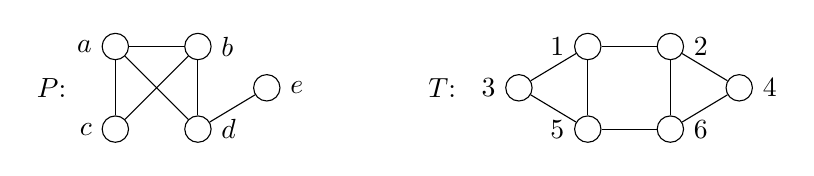
\begin{tikzpicture}
        \node[draw, circle, inner sep=0.5pt] (Na) at (0, 0) {\phantom{0}};
        \node[draw, circle, inner sep=0.5pt, right=0.7 of Na] (Nb) {\phantom{0}};
        \node[draw, circle, inner sep=0.5pt, below=0.7 of Na] (Nc) {\phantom{0}};
        \node[draw, circle, inner sep=0.5pt, right=0.7 of Nc] (Nd) {\phantom{0}};
        \node[draw, circle, inner sep=0.5pt, right=0.7 of $(Nb)!0.5!(Nd)$] (Ne) {\phantom{0}};
        \node[left=0 of Na] {$a$};
        \node[right=0 of Nb] {$b$};
        \node[left=0 of Nc] {$c$};
        \node[right=0 of Nd] {$d$};
        \node[right=0 of Ne] {$e$};
        \node[anchor=east, left=0.5 of $(Na)!0.5!(Nc)$] { $P$: };
        \draw (Na) -- (Nb);
        \draw (Na) -- (Nc);
        \draw (Na) -- (Nd);
        \draw (Nb) -- (Nc);
        \draw (Nb) -- (Nd);
        \draw (Nd) -- (Ne);

        \node[draw, circle, inner sep=0.5pt] (N1) at (6, 0) {\phantom{0}};
        \node[draw, circle, inner sep=0.5pt, right=0.7 of N1] (N2) {\phantom{0}};
        \node[draw, circle, inner sep=0.5pt, below=0.7 of N1] (N5) {\phantom{0}};
        \node[draw, circle, inner sep=0.5pt, below=0.7 of N2] (N6) {\phantom{0}};
        \node[draw, circle, inner sep=0.5pt, right=0.7 of $(N2)!0.5!(N6)$] (N4) {\phantom{0}};
        \node[draw, circle, inner sep=0.5pt, left=0.7 of $(N1)!0.5!(N5)$] (N3) {\phantom{0}};
        \node[left=0 of N1] {$1$};
        \node[right=0 of N2] {$2$};
        \node[left=0 of N3] {$3$};
        \node[right=0 of N4] {$4$};
        \node[left=0 of N5] {$5$};
        \node[right=0 of N6] {$6$};
        \node[anchor=east, left=0.5 of N3] { $T$: };
        \draw (N1) -- (N2);
        \draw (N1) -- (N3);
        \draw (N1) -- (N5);
        \draw (N2) -- (N4);
        \draw (N2) -- (N6);
        \draw (N3) -- (N5);
        \draw (N4) -- (N6);
        \draw (N5) -- (N6);
    \end{tikzpicture}

    \bigskip

    \bigskip

    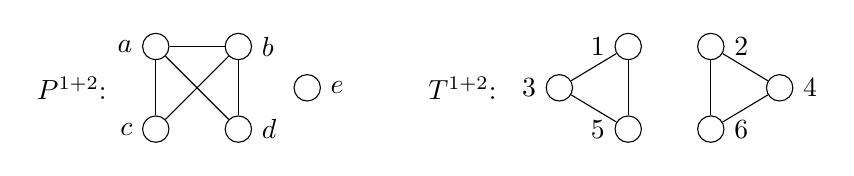
\begin{tikzpicture}
        \node[draw, circle, inner sep=0.5pt] (Ma) at (0, -2) {\phantom{0}};
        \node[draw, circle, inner sep=0.5pt, right=0.7 of Ma] (Mb) {\phantom{0}};
        \node[draw, circle, inner sep=0.5pt, below=0.7 of Ma] (Mc) {\phantom{0}};
        \node[draw, circle, inner sep=0.5pt, right=0.7 of Mc] (Md) {\phantom{0}};
        \node[draw, circle, inner sep=0.5pt, right=0.7 of $(Mb)!0.5!(Md)$] (Me) {\phantom{0}};
        \node[left=0 of Ma] {$a$};
        \node[right=0 of Mb] {$b$};
        \node[left=0 of Mc] {$c$};
        \node[right=0 of Md] {$d$};
        \node[right=0 of Me] {$e$};
        \node[anchor=east, left=0.5 of $(Ma)!0.5!(Mc)$] { $P^{1{+}2}$: };
        \draw (Ma) -- (Mb);
        \draw (Ma) -- (Mc);
        \draw (Ma) -- (Md);
        \draw (Mb) -- (Mc);
        \draw (Mb) -- (Md);

        \node[draw, circle, inner sep=0.5pt] (M1) at (6, -2) {\phantom{0}};
        \node[draw, circle, inner sep=0.5pt, right=0.7 of M1] (M2) {\phantom{0}};
        \node[draw, circle, inner sep=0.5pt, below=0.7 of M1] (M5) {\phantom{0}};
        \node[draw, circle, inner sep=0.5pt, below=0.7 of M2] (M6) {\phantom{0}};
        \node[draw, circle, inner sep=0.5pt, right=0.7 of $(M2)!0.5!(M6)$] (M4) {\phantom{0}};
        \node[draw, circle, inner sep=0.5pt, left=0.7 of $(M1)!0.5!(M5)$] (M3) {\phantom{0}};
        \node[left=0 of M1] {$1$};
        \node[right=0 of M2] {$2$};
        \node[left=0 of M3] {$3$};
        \node[right=0 of M4] {$4$};
        \node[left=0 of M5] {$5$};
        \node[right=0 of M6] {$6$};
        \node[anchor=east, left=0.5 of M3] { $T^{1{+}2}$: };
        \draw (M1) -- (M3);
        \draw (M1) -- (M5);
        \draw (M2) -- (M4);
        \draw (M2) -- (M6);
        \draw (M3) -- (M5);
        \draw (M4) -- (M6);
    \end{tikzpicture}\end{center}
\end{frame}

\begin{frame}{Induced Subisomorphisms}
    \begin{itemize}
        \item Find something that is a non-induced subisomorphism \[
                P \rightarrowtail T
            \] and simultaneously a non-induced subisomorphism \[
                \overline{P} \rightarrowtail \overline{T}
            \]
    \end{itemize}
\end{frame}

\begin{frame}{Partially Defined Graphs}
    \begin{itemize}
        \item Challenge for you!
    \end{itemize}
\end{frame}

\subsection{Kraiczy, McCreesh: Solving Graph Homomorphism and Subgraph Isomorphism Problems Faster Through Clique Neighbourhood Constraints. IJCAI 2021}

\begin{frame}{Clique Neighbourhood Filtering}
    \begin{itemize}
        \item If a pattern vertex is contained in a $k$-vertex clique, it must be mapped to a
            target vertex contained in at least a $k$-vertex clique.
        \item Valid without injectivity (with a caveat for loops).
    \end{itemize}

    \bigskip\centering
    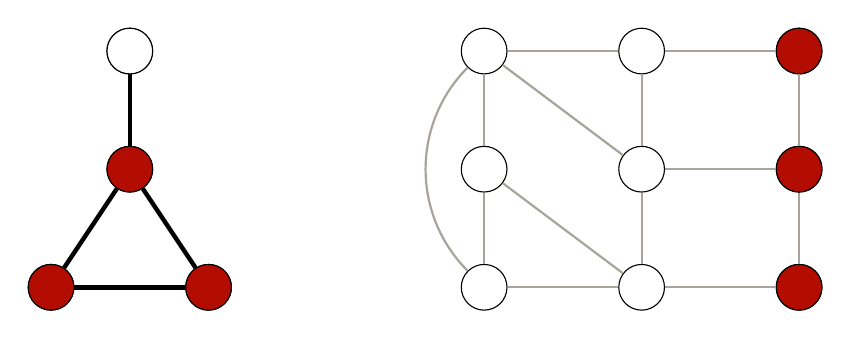
\begin{tikzpicture}
        \node <1> [draw, circle, fill=white, inner sep=4pt, font=\bfseries] (Na) at (1,  0) {\vphantom{1}};
        \node <1> [draw, circle, fill=white, inner sep=4pt, font=\bfseries] (Nb) at (1, -1.5) {\vphantom{1}};
        \node <1> [draw, circle, fill=white, inner sep=4pt, font=\bfseries] (Nc) at (0, -3) {\vphantom{1}};
        \node <1> [draw, circle, fill=white, inner sep=4pt, font=\bfseries] (Nd) at (2, -3) {\vphantom{1}};

        \node <2> [draw, circle, fill=white, inner sep=4pt, font=\bfseries] (Na) at (1,  0) {\vphantom{1}};
        \node <2> [draw, circle, fill=uofgpillarbox, inner sep=4pt, font=\bfseries] (Nb) at (1, -1.5) {\vphantom{1}};
        \node <2> [draw, circle, fill=uofgpillarbox, inner sep=4pt, font=\bfseries] (Nc) at (0, -3) {\vphantom{1}};
        \node <2> [draw, circle, fill=uofgpillarbox, inner sep=4pt, font=\bfseries] (Nd) at (2, -3) {\vphantom{1}};

        \draw [ultra thick] (Na) -- (Nb);
        \draw [ultra thick] (Nb) -- (Nc);
        \draw [ultra thick] (Nc) -- (Nd);
        \draw [ultra thick] (Nb) -- (Nd);

        \node [draw, circle, fill=white, inner sep=4pt, font=\bfseries] (N1) at (5.5,  0) {\vphantom{1}};
        \node [draw, circle, fill=white, inner sep=4pt, font=\bfseries] (N2) at (7.5,  0) {\vphantom{1}};
        \node [draw, circle, fill=white, inner sep=4pt, font=\bfseries] (N3) at (5.5, -1.5) {\vphantom{1}};
        \node [draw, circle, fill=white, inner sep=4pt, font=\bfseries] (N4) at (7.5, -1.5) {\vphantom{1}};
        \node [draw, circle, fill=white, inner sep=4pt, font=\bfseries] (N5) at (5.5, -3) {\vphantom{1}};
        \node [draw, circle, fill=white, inner sep=4pt, font=\bfseries] (N6) at (7.5, -3) {\vphantom{1}};

        \node <1> [draw, circle, fill=white, inner sep=4pt, font=\bfseries] (N7) at (9.5, -3) {\vphantom{1}};
        \node <2> [draw, circle, fill=uofgpillarbox, inner sep=4pt, font=\bfseries] (N7) at (9.5, -3) {\vphantom{1}};
        \node <1> [draw, circle, fill=white, inner sep=4pt, font=\bfseries] (N8) at (9.5, -1.5) {\vphantom{1}};
        \node <2> [draw, circle, fill=uofgpillarbox, inner sep=4pt, font=\bfseries] (N8) at (9.5, -1.5) {\vphantom{1}};
        \node <1> [draw, circle, fill=white, inner sep=4pt, font=\bfseries] (N9) at (9.5, 0) {\vphantom{1}};
        \node <2> [draw, circle, fill=uofgpillarbox, inner sep=4pt, font=\bfseries] (N9) at (9.5, 0) {\vphantom{1}};

        \draw [thick, color=uofgsandstone!50] (N1) -- (N2);
        \draw [thick, color=uofgsandstone!50] (N1) -- (N3);
        \draw [thick, color=uofgsandstone!50] (N1) -- (N4);
        \draw [thick, color=uofgsandstone!50] (N2) -- (N4);
        \draw [thick, color=uofgsandstone!50] (N3) -- (N5);
        \draw [thick, color=uofgsandstone!50] (N3) -- (N6);
        \draw [thick, color=uofgsandstone!50] (N4) -- (N6);
        \draw [thick, color=uofgsandstone!50] (N5) -- (N6);
        \draw [thick, color=uofgsandstone!50] (N1) to [in=135, out=225] (N5);

        \draw [thick, color=uofgsandstone!50] (N7) -- (N8);
        \draw [thick, color=uofgsandstone!50] (N8) -- (N9);
        \draw [thick, color=uofgsandstone!50] (N2) -- (N9);
        \draw [thick, color=uofgsandstone!50] (N4) -- (N8);
        \draw [thick, color=uofgsandstone!50] (N6) -- (N7);
    \end{tikzpicture}
\end{frame}

\section{Search}

\subsection{Archibald, Dunlop, Hoffmann, McCreesh, Prosser, Trimble: Sequential and Parallel Solution-Biased Search for Subgraph Algorithms.
CPAIOR 2019}

\begin{frame}{Variable and Value Ordering Heuristics}
    \begin{itemize}
        \item Variable ordering (i.e.\ pattern vertices): smallest domain first, tie-breaking on highest degree.
            \begin{itemize}
                \item Tends to pick vertices adjacent to things we've already picked.
            \end{itemize}
        \item Value ordering (i.e.\ target vertices): highest degree to lowest.
    \end{itemize}
\end{frame}

\begin{frame}{Sanity Check}
    \begin{center}
        \includegraphics<1>{gen-graph-value-ordering.pdf}
        \includegraphics<2>{gen-graph-value-ordering-unsat.pdf}
    \end{center}
\end{frame}

\begin{frame}{However\ldots}
    \begin{itemize}
        \item What if several vertices have the same degree?
        \item Is a vertex of degree $10$ really that much better than a vertex of degree $9$?
    \end{itemize}
\end{frame}

\begin{frame}{Random Search with Restarts and Nogood Recording}
    \only<1>{\begin{itemize}
        \item Back to the random value-ordering heuristic.
        \item Aggressive restarts: every 100ms.
        \item Nogood recording to avoid repeating work.
    \end{itemize}}\only<2->{
    \begin{center}
        \includegraphics<2>{gen-graph-rsr.pdf}%
    \end{center}}
\end{frame}


\begin{frame}{Value-Ordering Heuristics as Distributions}
    \begin{itemize}
        \item Traditional view: value-ordering defines a search order.
        \item New view: value-ordering defines \textcolor{uofgcobalt}{what proportion of the search
            effort} should be spent on different subproblems.
        \item According to people who know more statistics than me, if solutions are uniformly
            distributed, then random search with restarts should be better than DFS.
    \end{itemize}
\end{frame}

\begin{frame}{A Slightly Random Value-Ordering Heuristic}
    \only<1>{
    \begin{itemize}
        \item For a fixed domain $D_v$, pick a vertex $v'$ from a domain $D_v$ with probability
    \[ p(v') = \frac{2^{\deg(v')}}{\sum_{w \in D_v}{2^{\deg(w)}}} \]
        \item Equally likely to pick between two vertices of degree $d$.
        \item Twice as likely to select a vertex of degree $d$ than a vertex of degree $d - 1$.
        \item Justification: \textcolor{uofgcobalt}{solution density} and expected distribution of solutions.
    \end{itemize}}\only<2>{
    \begin{center}
        \includegraphics<2>{gen-graph-bias-scatter.pdf}%
    \end{center}}
\end{frame}

\begin{frame}{Is It Better?}
    \begin{center}
        \includegraphics<1>{gen-graph-sbs-scatter.pdf}%
        \includegraphics<2>{gen-graph-sbs.pdf}%
    \end{center}
\end{frame}

\begin{frame}{Parallel Search}
    \begin{itemize}
        \item Each thread gets its own random seed.
        \item Barrier synchronise on restarts.
        \item Share nogoods.
    \end{itemize}
\end{frame}

\begin{frame}{Is It Even Betterer?}
    \begin{center}
    \includegraphics<1>{gen-graph-par-scatter.pdf}%
    \includegraphics<2>{gen-graph-par.pdf}%
    \includegraphics<3>{gen-graph-dist.pdf}%
    \end{center}
\end{frame}

\section{Proof Logging}

\subsection{Gocht, McBride, McCreesh, Nordstr\"om, Prosser, Trimble: Certifying Solvers for Clique and Maximum Common (Connected) Subgraph Problems.
CP 2020}

\begin{frame}{Why Trust Solvers?}
    \begin{itemize}
        \item Solvers generally fairly reliable, but not perfect.
        \item Having solved a billion instances, error rate of 0.1\% in ``state of the
            art solver'' for maximum clique.
            \pause
        \item Obviously my solver is totally bug-free.
    \end{itemize}
\end{frame}

\begin{frame}{Proof Logging}
    \vspace*{-1.0em}
    \begin{center}
        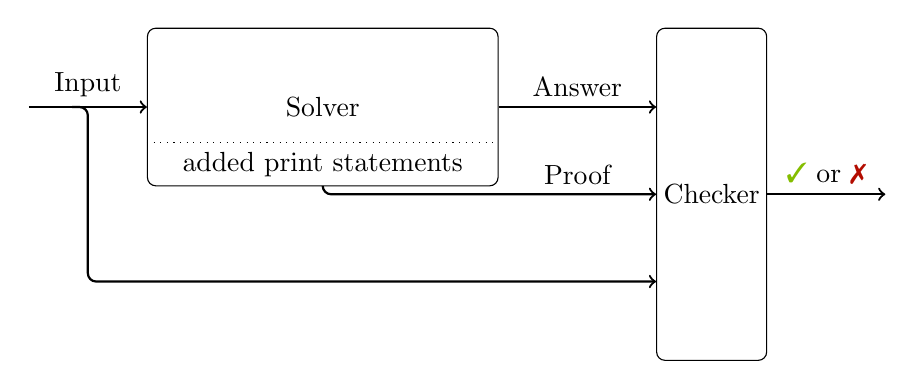
\begin{tikzpicture}
            \node (solver) [inner xsep=5em, inner ysep=2.5em, draw, rounded corners=3pt] { Solver };

            \node (checker) [right=2cm of solver.north east, anchor=north west, inner xsep=0.25em, draw, rounded corners=3pt, minimum height=12em, visible on=<3->] { Checker };

            \node (print) [anchor=south, above=0cm of solver.south, visible on=<2->] { added print statements };
            \draw [dotted, visible on=<2->] (solver.west|-print.north) -- (solver.east|-print.north);

            \draw [->, thick] (solver.east) -- (solver.east -| checker.west)
                coordinate [midway] (solutionmid) node [above, midway] { Answer };

            \draw [->, thick, rounded corners=3pt, visible on=<2->] (solver.south) -- (solver.south |- checker.west)
                -- (checker.west) coordinate [midway] (proofmid);

            \coordinate (prooflabel) at (proofmid-|solutionmid);
            \node [above=0cm of prooflabel, visible on=<2->] { Proof };

            \coordinate [right=1.5cm of checker.east] (verified);
            \draw [->, thick, visible on=<4->] (checker.east) -- (verified) node [above, midway] { \textcolor{uofglawn}{\ding{51}} or \textcolor{uofgpillarbox}{\ding{55}} };

            \coordinate [left=1.5cm of solver.west] (input);
            \draw [->, thick] (input) -- (solver.west) coordinate [midway] (inputmid) node [above, midway] { Input };

            \coordinate (checkerbotleft) at ($(checker.west)+($(checker.west)-(solver.east-|checker.west)$)$);

            \draw [->, thick, rounded corners=3pt, visible on=<3->] ($(inputmid)+(-0.2,0)$) -- (inputmid) -- (inputmid |- checkerbotleft) -- (checkerbotleft);
        \end{tikzpicture}
      \end{center}
    \vspace*{-0.7em}
  \begin{enumerate}
  \item<1->
    Run solver on problem input.
  \item<2->
    Solver also prints out a proof as part of its output.
  \item<3->
    Feed input + solution + proof to proof checker.
  \item<4->
    Verify that proof checker says solution is correct.
  \end{enumerate}
\end{frame}

\subsection{Bogaerts, Gocht, McCreesh, Nordstr\"om: Certified Dominance and Symmetry Breaking for
Combinatorial Optimisation. JAIR 77 (2023).}

\begin{frame}{The VeriPB Proof System}
    \begin{center}
        \url{https://gitlab.com/MIAOresearch/software/VeriPB}
    \end{center}

    \bigskip

    \begin{itemize}
        \item Built upon 0-1 integer linear inequalities: a superset of Boolean CNF.
        \item Doesn't know what graphs are\ldots
    \end{itemize}
\end{frame}

\subsection{Gocht, McCreesh, Nordstr\"om: Subgraph Isomorphism Meets Cutting Planes: Solving With Certified Solutions. IJCAI 2020}

\begin{frame}{A Slightly Different Workflow}
    \begin{center}
        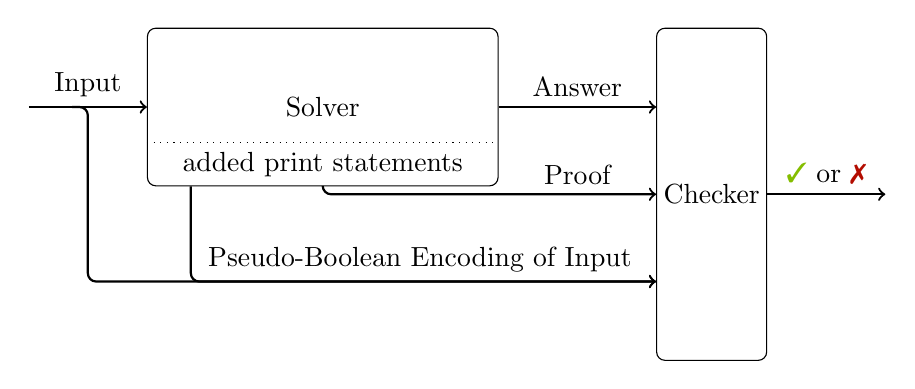
\begin{tikzpicture}
            \node (solver) [inner xsep=5em, inner ysep=2.5em, draw, rounded corners=3pt] { Solver };

            \node (checker) [right=2cm of solver.north east, anchor=north west,
            inner xsep=0.25em, draw, rounded corners=3pt, minimum height=12em, visible on=<3->] { Checker };

            \node (print) [anchor=south, above=0cm of solver.south, visible on=<2->] { added print statements };
            \draw [dotted, visible on=<2->] (solver.west|-print.north) -- (solver.east|-print.north);

            \draw [->, thick] (solver.east) -- (solver.east -| checker.west)
                coordinate [midway] (solutionmid) node [above, midway] { Answer };

            \draw [->, thick, rounded corners=3pt, visible on=<2->] (solver.south) -- (solver.south |- checker.west)
                -- (checker.west) coordinate [midway] (proofmid);

            \coordinate (prooflabel) at (proofmid-|solutionmid);
            \node [above=0cm of prooflabel, visible on=<2->] { Proof };

            \coordinate [right=1.5cm of checker.east] (verified);
            \draw [->, thick, visible on=<5->] (checker.east) -- (verified) node [above, midway] { \textcolor{uofglawn}{\ding{51}} or \textcolor{uofgpillarbox}{\ding{55}} };

            \coordinate [left=1.5cm of solver.west] (input);
            \draw [->, thick] (input) -- (solver.west) coordinate [midway] (inputmid) node [above, midway] { Input };

            \coordinate (checkerbotleft) at ($(checker.west)+($(checker.west)-(solver.east-|checker.west)$)$);

            \draw [->, thick, rounded corners=3pt, visible on=<3>] ($(inputmid)+(-0.2,0)$) --
            (inputmid) -- (inputmid |- checkerbotleft) -- (checkerbotleft) coordinate [midway] (altinputmid);
            \coordinate (solverstart) at ($(solver.south)!0.75!(solver.south west)$);
            \draw [->, thick, rounded corners=3pt, visible on=<4->] (solverstart) -- (solverstart |- checkerbotleft) -- (checkerbotleft);

            \coordinate (encinputlabel) at (altinputmid-|solutionmid);
            \node [above=0cm of encinputlabel, xshift=-2cm, visible on=<4->] { Pseudo-Boolean Encoding of Input };
        \end{tikzpicture}
    \end{center}
\end{frame}

\begin{frame}{So Far So Good\ldots}
    \begin{itemize}
        \item Lets us trust solutions\ldots
            \pause
        \item \ldots if you trust the encoding \ldots
            \pause
        \item \ldots and if you trust the proof checker \ldots
    \end{itemize}
\end{frame}

\subsection{Gocht, McCreesh, Myreen, Nordstr\"om, Oertel, Tan: End-to-End Verification for Subgraph Solving, AAAI 2024}

\begin{frame}{Reducing the Trust Base}
    \begin{center}
        \begin{tikzpicture}
            \node (solver) [ inner xsep=4em, inner ysep=2.5em, draw, rounded corners=3pt] { Solver };
            \node (elaborator) [ right=2cm of solver.north east, anchor=north west, inner
            xsep=0.25em, draw, rounded corners=3pt, minimum height=12em, text width=5em, text centered] {
                \only<1>{Checker}\only<2->{Elaborator} };
            \node (verifiedchecker) [ right=2cm of elaborator.north east, anchor=north west, inner
                xsep=0.25em, draw, rounded corners=3pt, minimum height=8em, text width=4em, text
                centered, yshift=-2cm, visible on=<3->] { Verified Checker };

            \node (print) [anchor=south, above=0cm of solver.south] { added print statements };
            \draw [dotted] (solver.west|-print.north) -- (solver.east|-print.north);

            \draw [->, thick] (solver.east) -- (solver.east -| elaborator.west) coordinate [midway]
            (solutionmid) node [above, midway] { Answer };

            \draw [->, thick, rounded corners=3pt] (solver.south) -- (solver.south |- elaborator.west) -- (elaborator.west) coordinate [midway] (proofmid);

            \coordinate (prooflabel) at (proofmid-|solutionmid); \node [above=0cm of prooflabel] { Proof };

            \coordinate [right=2cm of verifiedchecker.east] (verified);
            \draw [->, thick, visible on=<3>] (verifiedchecker.east) -- (verified)
                node [above, midway] { \textcolor{uofglawn}{\ding{51}} or \textcolor{uofgpillarbox}{\ding{55}} }
                node [below, midway, text centered, text width=5em] { Trusted Answer };
            \draw [->, thick, visible on=<4>] (verifiedchecker.east) -- (verified)
                node [above, midway] { \textcolor{uofglawn}{\ding{51}} or \textcolor{uofgpillarbox}{\ding{55}} }
                node [below, midway, text centered, text width=5em] { Trusted Answer in Graph Language };

            \coordinate [left=1.5cm of solver.west] (input);
            \draw [->, thick] (input) -- (solver.west) coordinate [midway] (inputmid) node [above, midway] { Input };

            \coordinate (verifiedcheckertopleft) at ($(verifiedchecker.west)+($(0cm,1.2cm)$)$);
            \draw [->, thick, visible on=<2->] (elaborator.east |- verifiedcheckertopleft) --
            (verifiedcheckertopleft) node [above, midway, text width=4em, text centered] { Answer };
            \draw [->, thick, visible on=<2->] (elaborator.east |- verifiedchecker.west) -- (verifiedchecker.west) node [above, midway, text width=4em, text centered] { Kernel Proof };

            \coordinate (elaboratorbotleft) at ($(elaborator.west)+($(elaborator.west)-(solver.east-|elaborator.west)$)$);
            \coordinate (verifiedcheckerbotleft) at ($(verifiedchecker.west)+($(0cm,-1.2cm)$)$);

            \coordinate (elaboratortopright) at ($(elaborator.east)+($(verifiedcheckertopleft)-(verifiedchecker.west)$)$);
            \draw [->, thick] (elaboratortopright) -- (elaboratortopright-|verifiedchecker.west)
                node [above, midway] { \textcolor{uofglawn}{\ding{51}} or \textcolor{uofgpillarbox}{\ding{55}} };

            \coordinate (solverstart) at ($(solver.south)!0.75!(solver.south west)$);
            \coordinate (checkerbotleft) at ($(elaborator.west)+($(elaborator.west)-(solver.east-|elaborator.west)$)$);
            \draw [->, thick, rounded corners=3pt] (solverstart) -- (solverstart |- checkerbotleft) -- (checkerbotleft)
            coordinate [midway] (altinputmid);

            \coordinate (encinputlabel) at (altinputmid-|solutionmid);
            \node [above=0cm of encinputlabel, xshift=-0.5cm] { Encoded Input };

            \draw [->, thick, rounded corners=3pt, visible on=<3>] (solverstart) -- (solverstart |- verifiedcheckerbotleft) -- (verifiedcheckerbotleft);
            \draw [->, thick, rounded corners=3pt, visible on=<4>] ($(inputmid)+(-0.2,0)$) --
            (inputmid) -- (inputmid |- verifiedcheckerbotleft) -- (verifiedcheckerbotleft)
            coordinate [midway] (verinputmid);

            \coordinate (verinputlabel) at (verinputmid-|solutionmid);
            \node [above=0cm of verinputlabel, xshift=-0.5cm, visible on=<4>] { Verified Input };
        \end{tikzpicture}
    \end{center}
\end{frame}

\begin{frame}[fragile]{End-to-End Verification of Subgraph-Finding}\vspace*{-0.3cm}
\begin{Verbatim}
$ glasgow_clique_solver brock200_4.clq --prove brock200_4 --proof-names --recover-proof-enc
omega = 17
clique = 12 19 28 29 38 54 65 71 79 93 117 127 139 161 165 186 192

$ veripb proof.opb proof.pbp
Verification succeeded.

$ grep conclusion proof.pbp
conclusion BOUNDS 183 183

$ cake_pb_clique brock200_4.clq > brock200_4.verifiedopb

$ veripb proof.verifiedopb proof.pbp --proofOutput proof.corepb
Verification succeeded.

$ cake_pb_clique brock200_4.clq proof.corepb
s VERIFIED MAX CLIQUE SIZE |CLIQUE| = 17
\end{Verbatim}
\end{frame}

\begin{frame}{What Exactly are we Verifying?}
    \only<1>{
    \begin{holthmenv}
    \HOLConst{is_clique}\;\HOLFreeVar{vs}\;(\HOLFreeVar{v}\HOLSymConst{,}\HOLFreeVar{e})\;\HOLTokenDefEquality{}\\
    \;\;\HOLFreeVar{vs}\;\HOLSymConst{\HOLTokenSubset{}}\;\HOLcount{\HOLFreeVar{v}}\;\HOLSymConst{\HOLTokenConj{}}\\
    \;\;\HOLSymConst{\HOLTokenForall{}}\HOLBoundVar{x}\;\HOLBoundVar{y}.\;\HOLBoundVar{x}\;\HOLSymConst{\HOLTokenIn{}}\;\HOLFreeVar{vs}\;\HOLSymConst{\HOLTokenConj{}}\;\HOLBoundVar{y}\;\HOLSymConst{\HOLTokenIn{}}\;\HOLFreeVar{vs}\;\HOLSymConst{\HOLTokenConj{}}\;\HOLBoundVar{x}\;\HOLSymConst{\HOLTokenNotEqual{}}\;\HOLBoundVar{y}\;\HOLSymConst{\HOLTokenImp{}}\;\HOLConst{is_edge}\;\HOLFreeVar{e}\;\HOLBoundVar{x}\;\HOLBoundVar{y}
    \end{holthmenv}

    \begin{holthmenv}
    \HOLConst{max_clique_size}\;\HOLFreeVar{g}\;\HOLTokenDefEquality{}\;\HOLConst{max\ensuremath{_{\text{set}}}}\;\HOLTokenLeftbrace{}\HOLConst{card}\;\HOLBoundVar{vs}\;\HOLTokenBar{}\;\HOLConst{is_clique}\;\HOLBoundVar{vs}\;\HOLFreeVar{g}\HOLTokenRightbrace{}
    \end{holthmenv}
}\only<2>{
\begin{holthmenv}
\HOLConst{clique_eq_str}\;\HOLFreeVar{n}\;\HOLTokenDefEquality{}\;\HOLStringLitDG{s VERIFIED MAX CLIQUE SIZE |CLIQUE| = }\;\HOLSymConst{\^{}}\;\HOLConst{toString}\;\HOLFreeVar{n}\;\HOLSymConst{\^{}}\;\HOLStringLitDG{\HOLTokenBackslash{}n}
\end{holthmenv}

\begin{holthmenv}
\HOLConst{clique_bound_str}\;\HOLFreeVar{l}\;\HOLFreeVar{u}\;\HOLTokenDefEquality{}\\
\;\;\HOLStringLitDG{s VERIFIED MAX CLIQUE SIZE BOUND }\;\HOLSymConst{\^{}}\;\HOLConst{toString}\;\HOLFreeVar{l}\;\HOLSymConst{\^{}}\;\HOLStringLitDG{ <= |CLIQUE| <= }\;\HOLSymConst{\^{}}\;\HOLConst{toString}\;\HOLFreeVar{u}\;\HOLSymConst{\^{}}\;\HOLStringLitDG{\HOLTokenBackslash{}n}
\end{holthmenv}

\begin{holthmenv}
\HOLTokenTurnstile{}\;\HOLConst{cake_pb_clique_run}\;\HOLFreeVar{cl}\;\HOLFreeVar{fs}\;\HOLFreeVar{mc}\;\HOLFreeVar{ms}\;\HOLSymConst{\HOLTokenImp{}}\\
\;\;\;\;\;\HOLConst{machine_sem}\;\HOLFreeVar{mc}\;(\HOLConst{basis_ffi}\;\HOLFreeVar{cl}\;\HOLFreeVar{fs})\;\HOLFreeVar{ms}\;\HOLSymConst{\HOLTokenSubset{}}\\
\;\;\;\;\;\;\;\HOLConst{extend_with_resource_limit}\;\HOLTokenLeftbrace{}\HOLConst{Terminate}\;\HOLConst{Success}\;(\HOLConst{cake_pb_clique_io_events}\;\HOLFreeVar{cl}\;\HOLFreeVar{fs})\HOLTokenRightbrace{}\;\HOLSymConst{\HOLTokenConj{}}\\
\;\;\;\;\;\HOLSymConst{\HOLTokenExists{}}\HOLBoundVar{out}\;\HOLBoundVar{err}.\\
\;\;\;\;\;\;\;\HOLConst{extract_fs}\;\HOLFreeVar{fs}\;(\HOLConst{cake_pb_clique_io_events}\;\HOLFreeVar{cl}\;\HOLFreeVar{fs})\;\HOLSymConst{=}\;\HOLConst{Some}\;(\HOLConst{add_stdout}\;(\HOLConst{add_stderr}\;\HOLFreeVar{fs}\;\HOLBoundVar{err})\;\HOLBoundVar{out})\;\HOLSymConst{\HOLTokenConj{}}\\
\;\;\;\;\;\;\;(\HOLBoundVar{out}\;\HOLSymConst{\HOLTokenNotEqual{}}\;\HOLStringLitDG{}\;\HOLSymConst{\HOLTokenImp{}}\\
\;\;\;\;\;\;\;\;\;\;\HOLSymConst{\HOLTokenExists{}}\HOLBoundVar{g}.\;\HOLConst{get_graph_dimacs}\;\HOLFreeVar{fs}\;(\HOLConst{el}\;\HOLNumLit{1}\;\HOLFreeVar{cl})\;\HOLSymConst{=}\;\HOLConst{Some}\;\HOLBoundVar{g}\;\HOLSymConst{\HOLTokenConj{}}\\
\;\;\;\;\;\;\;\;\;\;\;\;\;\;(\HOLConst{length}\;\HOLFreeVar{cl}\;\HOLSymConst{=}\;\HOLNumLit{2}\;\HOLSymConst{\HOLTokenConj{}}\;\HOLBoundVar{out}\;\HOLSymConst{=}\;\HOLConst{concat}\;(\HOLConst{print_pbf}\;(\HOLConst{full_encode}\;\HOLBoundVar{g}))\;\HOLSymConst{\HOLTokenDisj{}}\\
\;\;\;\;\;\;\;\;\;\;\;\;\;\;\;\HOLConst{length}\;\HOLFreeVar{cl}\;\HOLSymConst{=}\;\HOLNumLit{3}\;\HOLSymConst{\HOLTokenConj{}}\\
\;\;\;\;\;\;\;\;\;\;\;\;\;\;\;\;\;\;\;(\HOLBoundVar{out}\;\HOLSymConst{=}\;\HOLConst{clique_eq_str}\;(\HOLConst{max_clique_size}\;\HOLBoundVar{g})\;\HOLSymConst{\HOLTokenDisj{}}\\
\;\;\;\;\;\;\;\;\;\;\;\;\;\;\;\;\;\;\;\HOLSymConst{\HOLTokenExists{}}\HOLBoundVar{l}\;\HOLBoundVar{u}.\HOLBoundVar{out}\;\HOLSymConst{=}\;\HOLConst{clique_bound_str}\;\HOLBoundVar{l}\;\HOLBoundVar{u}\;\HOLSymConst{\HOLTokenConj{}}\;(\HOLSymConst{\HOLTokenForall{}}\HOLBoundVar{vs}.\;\HOLConst{is_clique}\;\HOLBoundVar{vs}\;\HOLBoundVar{g}\;\HOLSymConst{\HOLTokenImp{}}\;\HOLConst{card}\;\HOLBoundVar{vs}\;\HOLSymConst{\HOLTokenLeq{}}\;\HOLBoundVar{u})\;\HOLSymConst{\HOLTokenConj{}}\\
\;\;\;\;\;\;\;\;\;\;\;\;\;\;\;\;\;\;\;\;\;\;\;\;\;\;\HOLSymConst{\HOLTokenExists{}}\HOLBoundVar{vs}.\;\HOLConst{is_clique}\;\HOLBoundVar{vs}\;\HOLBoundVar{g}\;\HOLSymConst{\HOLTokenConj{}}\;\HOLBoundVar{l}\;\HOLSymConst{\HOLTokenLeq{}}\;\HOLConst{card}\;\HOLBoundVar{vs})))
\end{holthmenv}}
\end{frame}

\begin{frame}{What's Left to Trust?}
    Still have to trust:
    \begin{itemize}
        \item The HOL4 theorem prover.
        \item That the formal HOL model of the CakeML environment corresponds to the
            hardware on which it is run.
        \item HOL definition of what it means to be a maximum clique or a subgraph isomorphism.
        \item Input parsing and output formatting.
    \end{itemize}

    \bigskip

    No need to trust, or even know about:
    \begin{itemize}
        \item How the solver works.
        \item What pseudo-Boolean means.
    \end{itemize}
\end{frame}

\begin{frame}{Code}
  \begin{center}
    \url{https://github.com/ciaranm/glasgow-subgraph-solver}

      \bigskip

    \url{https://gitlab.com/MIAOresearch/software/VeriPB}

      \bigskip

      \url{https://gitlab.com/MIAOresearch/software/CakePB}
  \end{center}
\end{frame}

\section{Summary}

\begin{frame}{Lessons Learned}
    \begin{itemize}
        \item Got to get a lot of things right:
            \begin{itemize}
                \item Design.
                \item Engineering.
                \item Evaluation.
                \item Understanding the hardware.
            \end{itemize}
        \item Being clever only pays off if you can do it quickly.
            \begin{itemize}
                \item Except sometimes it pays off even if it's really expensive.
            \end{itemize}
        \item Not always clear what problem people really want to solve.
    \end{itemize}
\end{frame}

{
    \usebackgroundtemplate{
        \tikz[overlay, remember picture]
        \node[at=(current page.south), anchor=south, yshift=-1cm, inner sep=0pt]{\includegraphics[keepaspectratio=true, width=\paperwidth]{../../images/background2.jpg}};
    }

    \begin{frame}[plain,noframenumbering]
        \begin{tikzpicture}[remember picture, overlay]
            \node at (current page.north west) {
                \begin{tikzpicture}[remember picture, overlay]
                    \fill [fill=uofguniversityblue, anchor=north west] (0, 0) rectangle (\paperwidth, -2.8cm);
                \end{tikzpicture}
            };

            \node (logo) [anchor=north east, shift={(-0.8cm,-0.2cm)}] at (current page.north east) {
                
\includegraphics[keepaspectratio=true,scale=0.5]{../../images/UoG_keyline.pdf}
            };

            \node (logo2) [anchor=north, below=0.2cm of logo.south] {
                
\includegraphics[keepaspectratio=true,scale=0.1]{../../images/RAEngWhite.pdf}
            };

            \coordinate (logos) at ($(logo.south)!0.5!(logo2.north)$);

            \node [anchor=west, xshift=0.8cm] at (current page.west |- logos) {
                \begin{minipage}{0.60\paperwidth}\raggedright
                    \textcolor{white}{\url{https://ciaranm.github.io/}} \\[0.3cm]
                    \textcolor{white}{\href{mailto:ciaran.mccreesh@glasgow.ac.uk}{\nolinkurl{ciaran.mccreesh@glasgow.ac.uk}}}
                \end{minipage}
            };
        \end{tikzpicture}
    \end{frame}
}

\end{document}

